\documentclass[draft, jgrga]{agujournal2018}
\usepackage{apacite}
\usepackage{url}
% \usepackage[utf8]{inputenc}
\usepackage{amsmath}
\usepackage{multirow}
\usepackage{booktabs}
% \usepackage[font=normalsize]{caption}
\usepackage{threeparttable}
\journalname{JGR: Solid Earth}
\usepackage{siunitx}
% \linenumbers

\usepackage{ragged2e}

\usepackage[finalnew]{trackchanges}
% \usepackage{natbib}

\draftfalse


\author{Kelian Dascher-Cousineau}

\begin{document}
\large
\title{What controls variations in aftershock productivity?}

\authors{Kelian Dascher-Cousineau, Emily E. Brodsky, Thorne Lay, Thomas H. W. Goebel}


% \affiliation{1}{First Affiliation}
% \affiliation{2}{Second Affiliation}
% \affiliation{3}{Third Affiliation}
% \affiliation{4}{Fourth Affiliation}

\affiliation{}{University of California Santa Cruz, 1156 High Street
Earth and Planetary Sciences, Santa Cruz, CA 95064}
%(repeat as many times as is necessary)

%% Corresponding Author:
% Corresponding author mailing address and e-mail address:

% (include name and email addresses of the corresponding author.  More
% than one corresponding author is allowed in this LaTeX file and for
% publication; but only one corresponding author is allowed in our
% editorial system.)

% Example: \correspondingauthor{First and Last Name}{email@address.edu}

\correspondingauthor{Kelian Dascher-Cousineau}{kdascher@ucsc.edu}

%% Keypoints, final entry on title page.

%  List up to three key points (at least one is required)
%  Key Points summarize the main points and conclusions of the article
%  Each must be 100 characters or less with no special characters or punctuation

% Example:
% \begin{keypoints}
% \item	List up to three key points (at least one is required)
% \item	Key Points summarize the main points and conclusions of the article
% \item	Each must be 100 characters or less with no special characters or punctuation
% \end{keypoints}


\begin{keypoints}
\item The volume of available brittle lithosphere appears to be the primary control on aftershock productivity.
\item Lithosphere age, plate boundary type, normalized rupture area, aspect ratio, and dip  \change{significantly influence}{correlate with} aftershock productivity.
\item Statistical models based on multiple parameters significantly improve aftershock forecasts.
\end{keypoints}

\newpage

\justify

\section*{Abstract}

\remove{Earthquake aftershocks are nearly ubiquitous.} The number of aftershocks increases with mainshock size following a well-defined scaling law. However, excursions from the average behavior are common. This variability is particularly concerning for large earthquakes where the number of aftershocks varies by factors of 100 for mainshocks of comparable magnitude. Do observable factors lead to differences in aftershock behavior? We examine aftershock productivity relative to the global average for all mainshocks ($M_W>6.5$) from 1990 to 2019. A global map of earthquake productivity highlights the influence of tectonic regimes. Earthquake depth, lithosphere age and plate boundary type correspond well with earthquake productivity. We investigate the role of source attributes by compiling source dimensions, radiated seismic energy, new measurements of stress drop, and a novel measure of slip heterogeneity based on finite fault source inversions for the largest earthquakes from 1990 to 2017. \add{Stress drop, normalized rupture width, and aspect ratio correlate with aftershock productivity.}\remove{Particularly long and narrow, and high stress drop ruptures have lower productivity.} A machine learning method shows that a particular set of parameters (dip, lithospheric age and normalized rupture area) combines well to improve predictions of aftershock productivity on a cross-validated data set. Our overall analysis is consistent with a model where the volumetric abundance of nearby stressed faults controls the aftershock productivity rather than variations in source stress. The insights from this study shed light on an approach to forecasting relative productivity based on geological and rupture properties rather than \change{empirical}{local} calibration.

\section{Introduction}

Earthquakes cluster in time and space. In a typical sequence, the largest earthquake is the mainshock, those preceding are foreshocks, and those following are aftershocks \citep{Omori1895}. The clustering behavior is well-described by three statistical relationships characterizing the temporal- and size-distributions of earthquakes. \citep[e.g.,][]{Ogata1988}. The aftershock productivity law, which is sometimes known as the Reasenberg-Jones Law is

\begin{linenomath*}
\begin{equation}\label{eq:productivity}
    N(M)=k10^{\alpha M}
\end{equation}
\end{linenomath*}
%
where $N$ is the number of aftershocks, $M$ is the mainshock magnitude, and $k$ is a constant of proportionality \change{which subsumes the tendency to generate aftershocks and the magnitude of completeness of the earthquake catalog}{which depends on the number of aftershocks
per mainshock above the catalog completeness level} \citep{Reasenberg1989}. The productivity law fits a wide range of data with $\alpha\approx1$ \citep{Reasenberg1989, Yamanaka1990scalingshock,  DeArcangelis2016, Kisslinger1996,Tahir2015,Tahir2014Aftershock2005, Page}. Thus the basic phenomenon of an increasing number of aftershocks with increasing mainshock magnitude is captured and quantified empirically.

    \begin{figure}
        \centering
        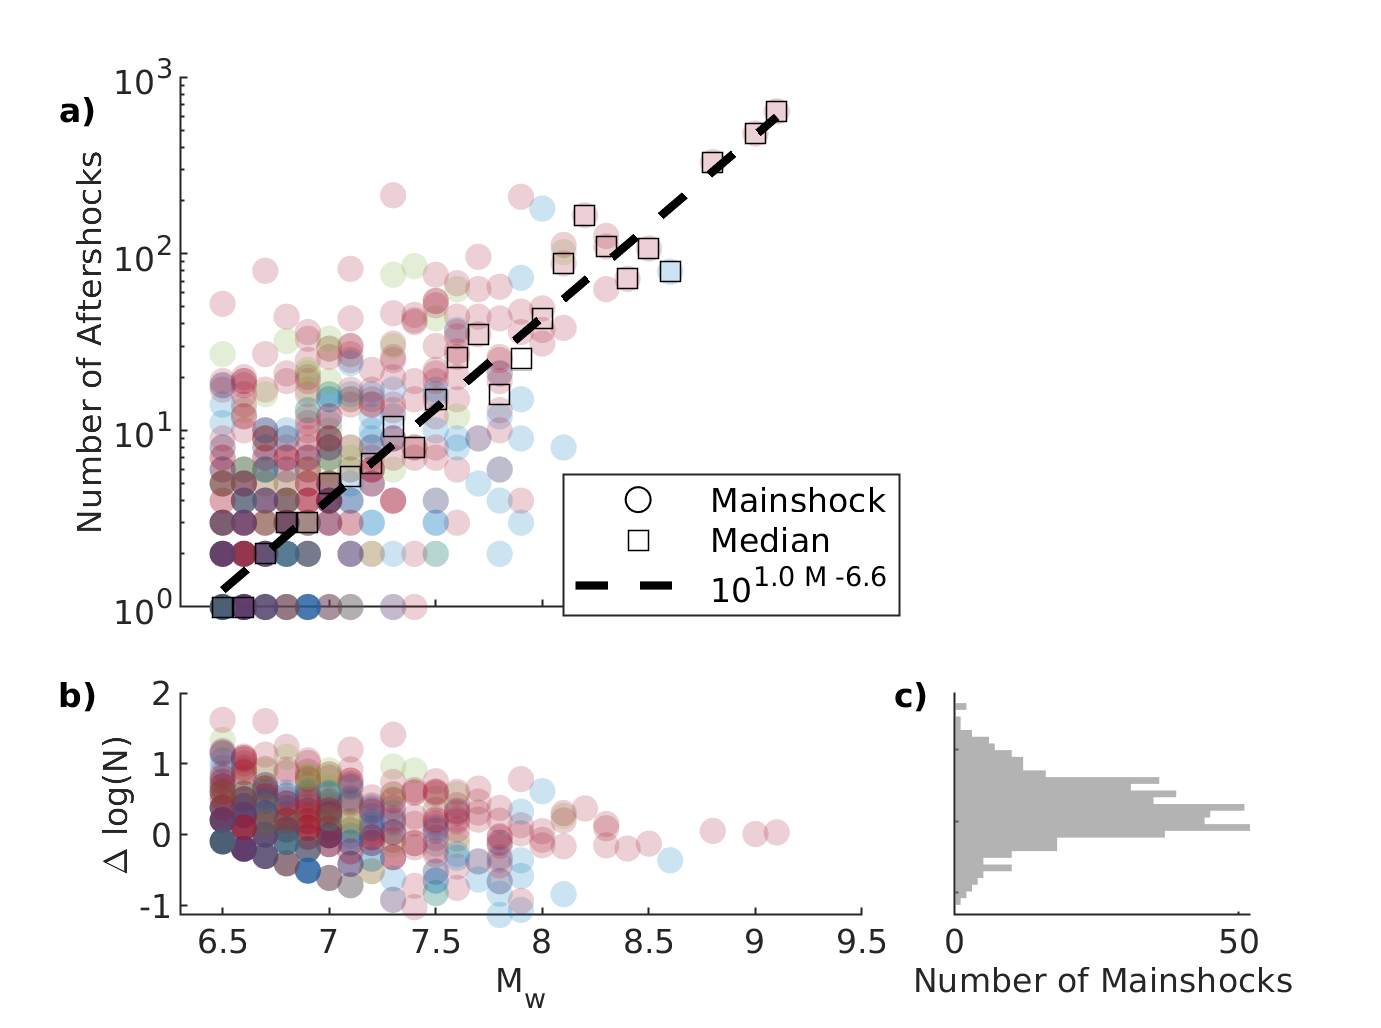
\includegraphics{prod_law.png}
        \caption{a) The number of aftershocks of $M_W\ge4.5$ within three source dimensions and 60 days as a function of mainshock magnitude identified in the global ISC and NEIC catalogs from 1990 to 2019. Colors indicate faulting style of the mainshock; blue, green and red points correspond to earthquake sequences for which the mainshock was respectively strike-slip, normal or reverse. The global productivity law (dashed line) is fit using a least squares regression through the median log-number of aftershocks for each 0.1 magnitude bin (black squares). The median number includes mainshocks with no aftershocks which are not shown on the plot. \add{Light dashed lines indicate 95\% confidences bounds given a Poisson distribution.} Individual earthquake sequences (circles) scatter significantly beyond these confidence limits. b) Relative productivity (Eq.~\ref{eq:residual_productivity}) as a function of mainshock magnitude. The relative productivity distribution does not show events with no aftershocks and thus the lower left corner of the plot is underpopulated. c) Histogram of the relative productivity of mainshocks considered in this study.
        }
        \label{fig:fms_prod}
    \end{figure}

\remove{Significant variations occur relative to the productivity law.} Figure \ref{fig:fms_prod}a shows 100-fold differences in the number of aftershocks for events of similar magnitude\add{ and far exceed 95\% confidence bounds that may be predicted from Poisson distribution given the rate predicted by} Equation~\ref{eq:productivity}. Such excursions from the scaling relationship are well documented by prior work \citep[e.g.][]{Marsan2017HowAftershocks,Boettcher2004EarthquakeFaults,Page,Tahir2014Aftershock2005}. Are these variations stochastic and unpredictable, or are they determined by features of particular sites or earthquakes?

The answer has practical consequences. Aftershock forecasting is currently the only operational form of earthquake prediction and is routinely used in the wake of major earthquakes to advise on short-term hazard following an earthquake \citep{Reasenberg1989, Page,Hardebeck2018UpdatedParameters}. Within a sequence, the probability of subsequent earthquakes exceeding the magnitude of the mainshock relates directly to the productivity \citep{Reasenberg1989, Reasenberg1999ForeshockEarthquakes}. Currently, variability in aftershock productivity is calibrated regionally where data permit or extrapolated from nearby regions and updated over the course of the aftershock sequence \citep[e.g.][]{Reasenberg1989, Reasenberg1999ForeshockEarthquakes, ogata2017statistics}. Many of these forecasts are empirical statistic models and, notably, rely heavily on high quality seismic data both before and during the earthquake \citep{Gerstenberger2005Real-timeCalifornia, Omi2015Intermediate-termApproaches}. \add{Other models embed physics-based rules that rely on local information about long term seismicity, the state of stress and the geometry of the faults} \citep[e.g.][]{Field2017AForecast}. \add{All of these approaches raise the critical issue of calibrating hazard in poorly instrumented areas.}

Yet previous studies have found that features related to the setting of the mainshock can inform aftershock abundance. Both global and regional studies indicate that tectonic regions have distinct aftershocks statistics \citep{Chu2011, Page, Davidsen2015GeneralizedCalifornia, Tahir2014Aftershock2005, ogata2017statistics}. For instance, the Eastern Pacific has greater aftershock productivity than the Western Pacific \citep{Singh1911, Wetzler2016}. Seismotectonic subdivisions (plate boundaries, global geology, seismicity catalogs, and regional and local studies) yield 10-fold differences in aftershocks productivity \citep{Page}. Active non-subduction continental regions have elevated earthquake productivity and, on average, larger aftershocks \citep{Page, Mogi1967, Davis1991Single-linkVariations}. In contrast, ridge transform faults are deficient in aftershocks \citep{Davis1991Single-linkVariations, Boettcher2004EarthquakeFaults, McGuire2005}. The local geological structure is thought to underlie these distinctions \citep{Boettcher2004EarthquakeFaults, McCloskey2003StructuralAftershocks}. \citet{Yamanaka1990scalingshock} report intraplate earthquakes as more productive than plate boundary earthquakes. \citet{Zaliapin2016AClusters} \add{find similar geographic patterns in clustering statistics and relate them to global heat flow.} Case studies generally reinforce the importance of geological structures on the distribution and intensity of aftershocks \citep{Das2003SpatialDistribution, McCloskey2003StructuralAftershocks}. An extreme case comes from deep focus subduction zone earthquakes, which sometimes generate few or no observable aftershocks \citep{Bath1965LateralMantle, Frohlich1989TheEarthquakes, Nyffenegger2000, Wiens1997AftershockZone, Wu1999, Houston2004}. Some work attributes the deficiency to the elevated temperature at depth \citep{Nyffenegger2000, Houston2004}.

Other studies elucidate the importance of source effects. Theoretical arguments, supported by systematics in the variance of stress drop measurements and earthquake productivity, have suggested that increased stress drop should correspond to increased productivity for Californian seismicity \citep{Marsan2017HowAftershocks}. The opposite relationship was documented for recent (1990-2016) major megathrust ruptures ($M_W \ge 7$) \citep{Wetzler2016}. The authors suggested that high stress drop corresponds to a smaller rupture area and therefore fewer aftershocks. This is supported by a tendency for megathrust aftershocks to occur on the periphery of large-slip zones \citep{Wetzler2016}. Earthquakes rupturing at supershear velocities also appear to have low aftershock productivity \citep{Bouchon2008TheEarthquakes}. A relationship between the heterogeneity of a rupture and the number of aftershocks has been a long-standing contention \citep{Mogi1967, Yamanaka1990scalingshock} with some support from rate and state models \citep{Helmstetter2006RelationModel, Marsan2006}, but few direct and quantitative measurements \citep{Das2003SpatialDistribution, Houston2004}. Finally, occurrence of dynamic triggering would suggest that radiated energy should influence the number of aftershocks \citep{felzer2006decay}.

Some observations cannot be distinctly associated with setting or source. There is a relationship between relative aftershock productivity and focal mechanism. Strike-slip earthquakes are proposed to be intrinsically less productive than dip-slip earthquakes \citep{Tahir2012, Tahir2014Aftershock2005, Tahir2015}. However, since strike-slip earthquakes occur in certain regions, it is unclear whether the reduced productivity is a site or source effect.

% Roadmap paragraph
\add{These studies elucidate the potential to use insight gathered globally to calibrate forecasts locally. Yet} the diversity in methods and data sets hinder an assessment of the relative importance of the above inferences. The goal of this paper is to systematically assess both setting and source effects on relative aftershock productivity and distill them down to significant parameters and then use this data to examine constraints on physical controls of aftershock productivity.  The calibration of productivity to physical factors begins to point the way towards an alternative approach to aftershock assessment on a global basis.

In this study, we first present a method of measuring relative aftershock productivity and defining a metric. We then provide an overview of global patterns in earthquake productivity, systematically addressing setting and source effects. We consider setting effects such as plate boundary type, depth, and lithospheric age; and source effects such as radiated energy, stress drop, source geometry, and slip heterogeneity. \add{Apparent correlations are compared to randomized catalogs to establish significance levels and we address the potential to generate spurious correlations because of the large number of attributes considered.} We attempt to disentangle site versus source focal mechanism influences using nearly co-located events. Machine learning tools establish a parsimonious set of parameters that can help in aftershock prediction and be used to improve our understanding of the physical controls on aftershock generation. Results indicate that the geometry of the source and the corresponding volumetric availability of stressed faults determine variations in earthquake productivity.

\section{Metrics and Data}

\subsection{Earthquake Catalogs and Investigated Parameters}

\add{To examine variations in aftershock productivity,} we utilize the National Earthquake Information Center (NEIC) for recent events and the International Seismological Center (ISC) locations and magnitudes as available for events from 1990 to 2019. We select earthquakes with moment magnitude exceeding global catalog completeness. \change{, $M_W4.5$, as determined by the first local minimum of a Kolmogorov-Smirnov test.}{We determine a global completeness utilizing the Kolmogorov-Smirnov test to evaluate the goodness of fit between a theoretical Gutenberg-Richter distribution and the data for a range of possible completeness magnitude}. We identify catalog completeness as the lowest earthquakes magnitude producing a local minimum in the Kolmogorov-Smirnov metric \citep[following][]{Clauset2009Power-lawData, Goebel2017WhatExperiments}.\add{ We test the sensitivity of our results to the magnitude of
completeness, finding consistent results for $M_c= 4.5$ to $5$ (Supplement figures S5-15)}.

%The Kolmogorov-Smirnov test measures   the similarity of distribution by computing the maximum distance between two distributions. Theoretical and observed distributions are similar if this Kolmogorov-Smirnov distance is small.
% Globally, we find that the completeness is  $M_W4.5$.} \add{Regional biases in catalog completeness directly influence the estimation of aftershock productivity. To ensure that these biases do not influence our major results, we include} supplement Figures S5 to S15 which reproduce this study's results using a more conservative completeness estimate of $M_W5$ \add{for near-total detection}.

We compare relative aftershock productivity to parameters that include site effects and source effects. Table \ref{tbl:attributes} outlines the selected attributes, coverage, and corresponding data sources. Locations, focal mechanism solutions, and radiated energy estimates were all obtained from the Incorporated Research Institutions for Seismology (IRIS) data management center and merged using earthquake identification numbers. Finite fault inversions produced and cataloged by \citet{Hayes2017} were associated with an aftershock statistic using a standardized Euclidean distance ($M_W$, latitude, longitude, depth, time).
Data and analytical limitations are such that rupture properties and source geometry are only available for 98 mainshocks with $M_W\ge6.8$ \citep{Hayes2017}. Supplement Table S1 includes the source attributes for these mainshocks. We treat multi-segmented rupture separately.

For several attributes, we scale the parameters in an effort to remove magnitude dependence. For instance, radiated energy is normalized by moment. We normalize width and length by the standard empirical length-scaling, $10^{0.59M_W}$ \citep[][Table 2A - Subsurface rupture dimensions]{Wells1994}. \add{We normalize rupture area correspondingly, $10^{0.91M_W}$} \citep[][Table 2A - Rupture area]{Wells1994}. Finally, we log-transform all of these values to linearize their distributions.

Following recommendations of \citet{Noda2013}, we compute stress drop measurements for all single plane finite fault inversions. Smoothing constraints on the finite fault inversions imply that the stress drop measurements are likely a lower, but consistent bound \citep{Adams2017ExploringInversions}.

Finally, we introduce a novel quantification of slip heterogeneity ($H$) derived from finite fault inversions. The metric compares the observed slip to a smooth reference slip distribution,
%
\begin{linenomath*}
\begin{equation}
    H = \dfrac{\mu \int_\Sigma |u-u_{ref}| dS}{M_o},
\end{equation}
\end{linenomath*}
%
where $\mu$ is the shear modulus, $u$ is the observed slip distribution, $u_{ref}$ is a reference slip distribution, $dS$ is an area element on the fault, $\Sigma$ is the entire finite fault area, and $M_o$ is the earthquake moment. The reference slip is prescribed as a positive ellipsoid fit to the slip distribution defined by free parameters $u_{c}, x_0, y_0, a$ and $b$,
%
\begin{linenomath*}
\begin{equation}\label{eq:heterogeneity}
u_{ref}=\left\{
\begin{array}{@{}ll@{}}
     \sqrt{u_{c}^2 - \left(\dfrac{x-x_0}{a}\right)^2 +  \left(\dfrac{y-y_0}{b}\right)^2}, & \text{if}\ \left(\dfrac{x-x_0}{a}\right)^2 +  \left(\dfrac{y-y_0}{b}\right)^2 < 1 \\
     \\
    0, & \text{otherwise}
    \end{array}\right.
\end{equation}
\end{linenomath*}
%
The heterogeneity measurement is designed to be most sensitive to large slip fluctuations such as asperities or barriers.

\begin{table}[]
\caption{Attributes considered in this study.}
\label{tbl:attributes}

\begin{threeparttable}
\centering
\setlength{\tabcolsep}{5.5pt}
\renewcommand{\arraystretch}{1.3}
\linespread{0.6}\selectfont\centering

\begin{tabular}{@{}lp{2cm}p{1cm}ccp{6.5cm}@{}}
\toprule
          & \textbf{Attributes}             & \multicolumn{3}{c}  {\textbf{Coverage}}  & \textbf{Comments}                                                                                                                                                                                          \\ \cmidrule(lr){3-5}
          &                                 & Spatial      & $M_c$ & Mainshocks  &                                                                                                                                                                                                            \\ \midrule
\multicolumn{2}{l}{\textbf{Site effects}}   &              &       &      &                                                                                                                                                                                                            \\
          & Time-location\tnote{1}          & Global       & 4.5   & 1011 &                                                                                                                                                                                                            \\
          & Plate boundaries\tnote{2}       & Global       & -     & 1011 & Categorized by nearest digitized boundary provided the focal mechanism is congruent\tnote{7} \hspace{1mm} for earthquakes $<$ 400 km from plate boundary; others are intraplate.                                                \\
          & Plate age and velocity\tnote{3} & Ocean basins & -     & 268  & Determined by nearest crustal age measurement up to 30 km from the mainshock.                                                                                                                                  \\
        %   & Lithospheric thickness\tnote{4} & Global       & -     & 2662 &                                                                                                                                                                                                            \\
\multicolumn{2}{l}{\textbf{Source effects}} &              &       &      &                                                                                                                                                                                                            \\
          & Radiated Energy\tnote{5}        & Global       & 6.0   &      &                                                                                                                                                                                                            \\
          & Source dimensions\tnote{6}      & Global       & 7.0   & 98   & Width (along-dip), length (along-strike) and aspect ratio of ruptures determined from autocorrelation width of finite fault inversions \citep[following][]{mai2000}. See text for notes on scaling.                                 \\
          & Rupture duration and velocity\tnote{7}& Global  & 7.0   & 98   &                                                                                                                                                                                                            \\
          & Material properties\tnote{7}    & Global       & 7.0   & 98   & $V_p$, $V_s$ and density used for inversions                                                                                                                                                         \\
          & Stress drop\tnote{6}            & Global       & 7.0   & 98   & See text                                                                                                                                                                                                  \\
          & Heterogeneity\tnote{6}          & Global       & 7.0   & 98   & See text, Equation \ref{eq:heterogeneity}                                                                                                                                                                                                   \\
\multicolumn{2}{l}{\textbf{Mixed effects}}  &              &       &      &                                                                                                                                                                                                            \\
          & Faulting style\tnote{8}         & Global       & 5.5   & 1011 & Categorized as strike-slip, normal, and reverse using the P and T axes                                                                                                                                     \\ \midrule
          &                                 &              & Total & 1011 &
\end{tabular}%

    \begin{tablenotes}
        \item[1] National Earthquake Information Center (NEIC) and International Seismological Centre (ISC) catalogs downloaded from the Incorporated Research Institutions for Seismology (IRIS) data management service.
        \item[2] \citet{Bird2003AnBoundaries}
        \item[3] \citet{Muller2008}
        % \item[4] \citet{Pasyanos2014LITHO1.0:Earth}
        \item[4] Produced by \citet{Convers2011GlobalMid2010} and downloaded from the Incorporated Research Institutions for Seismology (IRIS) data management service.
        \item[5] Attributes were derived from finite fault inversions produced by \citet{Hayes2017}.
        \item[6] Attributes directly measured by \citet{Hayes2017}.
        \item[7] Harvard global Centroid Moment Tensor Solutions (gCMT) and National Earthquake Information Center (NEIC) focal mechanism solutions downloaded from the Incorporated Research Institutions for Seismology (IRIS) data management service.

    \end{tablenotes}

\end{threeparttable}

\end{table}
%%%%%%%%%%%%%%%%%%%%%%%%%%%%%%%%%%%%%%%%%%%%%%%%%%%%%%%%%%%%%%%%%%%%%%%%%%%%%



    \subsection{Measuring Aftershock Productivity}

This study requires a consistent measure of aftershock productivity comparable on a global basis. To this end, we use a space-time windowing method to identify and count aftershocks. The event-level questions focusing on variations from the mean behavior examined here do not favor methods adaptively fitting different time or space periods and other seismicity parameters \citep[e.g.][]{ogata2017statistics}. \add{However, any aftershock counting method is subject to biases. We also utilize the clustering method of} \citet{Zaliapin2008} \add{as an alternative to test the robustness of our results to the chosen aftershock counting approach (see Supplement Section S1.3; Figures S16-25).}


For our primary windowing method, we classify earthquakes as foreshocks, mainshocks or aftershocks in a hierarchical sense \citep[following][]{felzer2006decay, Brodsky2011TheForeshocks, Wetzler2016, Garza-Giron2018Mainshock-AftershockRegions}. We define the largest earthquake in the catalog as a mainshock and then mark as foreshocks and aftershocks earthquakes within magnitude-dependent space and fixed time windows before and after the mainshock. The identified foreshocks and aftershocks are removed from further consideration to prevent double counting. A larger space and time window is used to ensure separation of sequences. Earthquakes within this larger window are also removed from consideration as potential mainshocks and do not count as aftershocks. We sequentially proceed to smaller mainshocks with this classification of foreshocks and aftershocks until we exhaust the catalog. The method is not designed to capture absolutely every aftershock, but rather to provide a consistent measure of aftershock productivity of each isolated mainshock. \add{For the purpose of our study, we only consider mainshocks with $M_W\ge6.5$ to ensure that the majority of analysed sequences have observable aftershocks.} \add{The hierarchical approach captures both mainshocks that arise naturally from background seismicity, and mainshocks in more complex chains of seismicity in which later earthquakes in a sequence become the largest earthquake and thus the mainshock.}

Specific trade-offs determine the choice of the time and space windows. Smaller windows increase the confidence that aftershocks are correctly attributed; conversely, larger time windows include more aftershocks and limit the effect of censored statistics (mainshocks with no aftershocks). We balance these trade-offs to find window selection criteria that yield the standard productivity relationships over the analyzed magnitude range (Figure~\ref{fig:sensitivity}). We assess the performance of each space-time window by comparing the results to the median of 100 time-shuffled catalogs that preserves the original spatial distribution but break the actual time sequence of the catalog \citep{Garza-Giron2018Mainshock-AftershockRegions}. The space-time window that includes the most aftershocks while separating the actual aftershock productivity relationship from the shuffled ones is the preferred choice.

Figure~\ref{fig:sensitivity} shows results for a suite of space and time windows. Space windows are all measured in terms of source radius estimated following Table 2A of \citet{Wells1994} \add{, which provides the subsurface rupture length}:
%
\begin{linenomath*}
\begin{equation}\label{eq:wells}
    R_{source}\sim (2\times 10^{0.59M_W})\SI{}{\meter}
\end{equation}
\end{linenomath*}
%
For reference, $M_W$ 6 and 9 earthquakes have dimensions on the order of $\sim 7$ km and $\sim 400$ km respectively. \add{We also check the results by using the more recent geodetic-derived scaling relationship of} \citet{Brengman2019EarthquakeScalingDistributions}.\add{ Supplemental Figure S2 demonstrates that the results are nearly the same with 79\% of the mainshocks having identical aftershock counts. A spherical space window of three source dimensions in radius centered on the mainshock location and a time window of 60 days following the mainshock performs best. Smaller and shorter windows result in a clearer separation of the shuffled statistic. However, the number of mainshocks with no aftershocks increases dramatically (e.g., 30\% of mainshocks in the case of the ten-day and one source dimension window, as opposed to 10\% for the our selected window). The larger space window, used to eliminate events from further consideration, is four source dimensions and an additional 40 days. We use the same combination of selection and screening in space window and 1 day time window to classify foreshocks. Using the space-time windowing approach we ensure that nearly all mainshocks (99\%) are fully isolated in time and space from each other. The non-isolated cases occur when two mainshocks of different magnitudes have overlapping, but not coincident, aftershock sequences. These occurrences are rare ($1\%$) and therefore we do not complicate the algorithm further to eliminate them.}

\begin{figure}
    \centering
    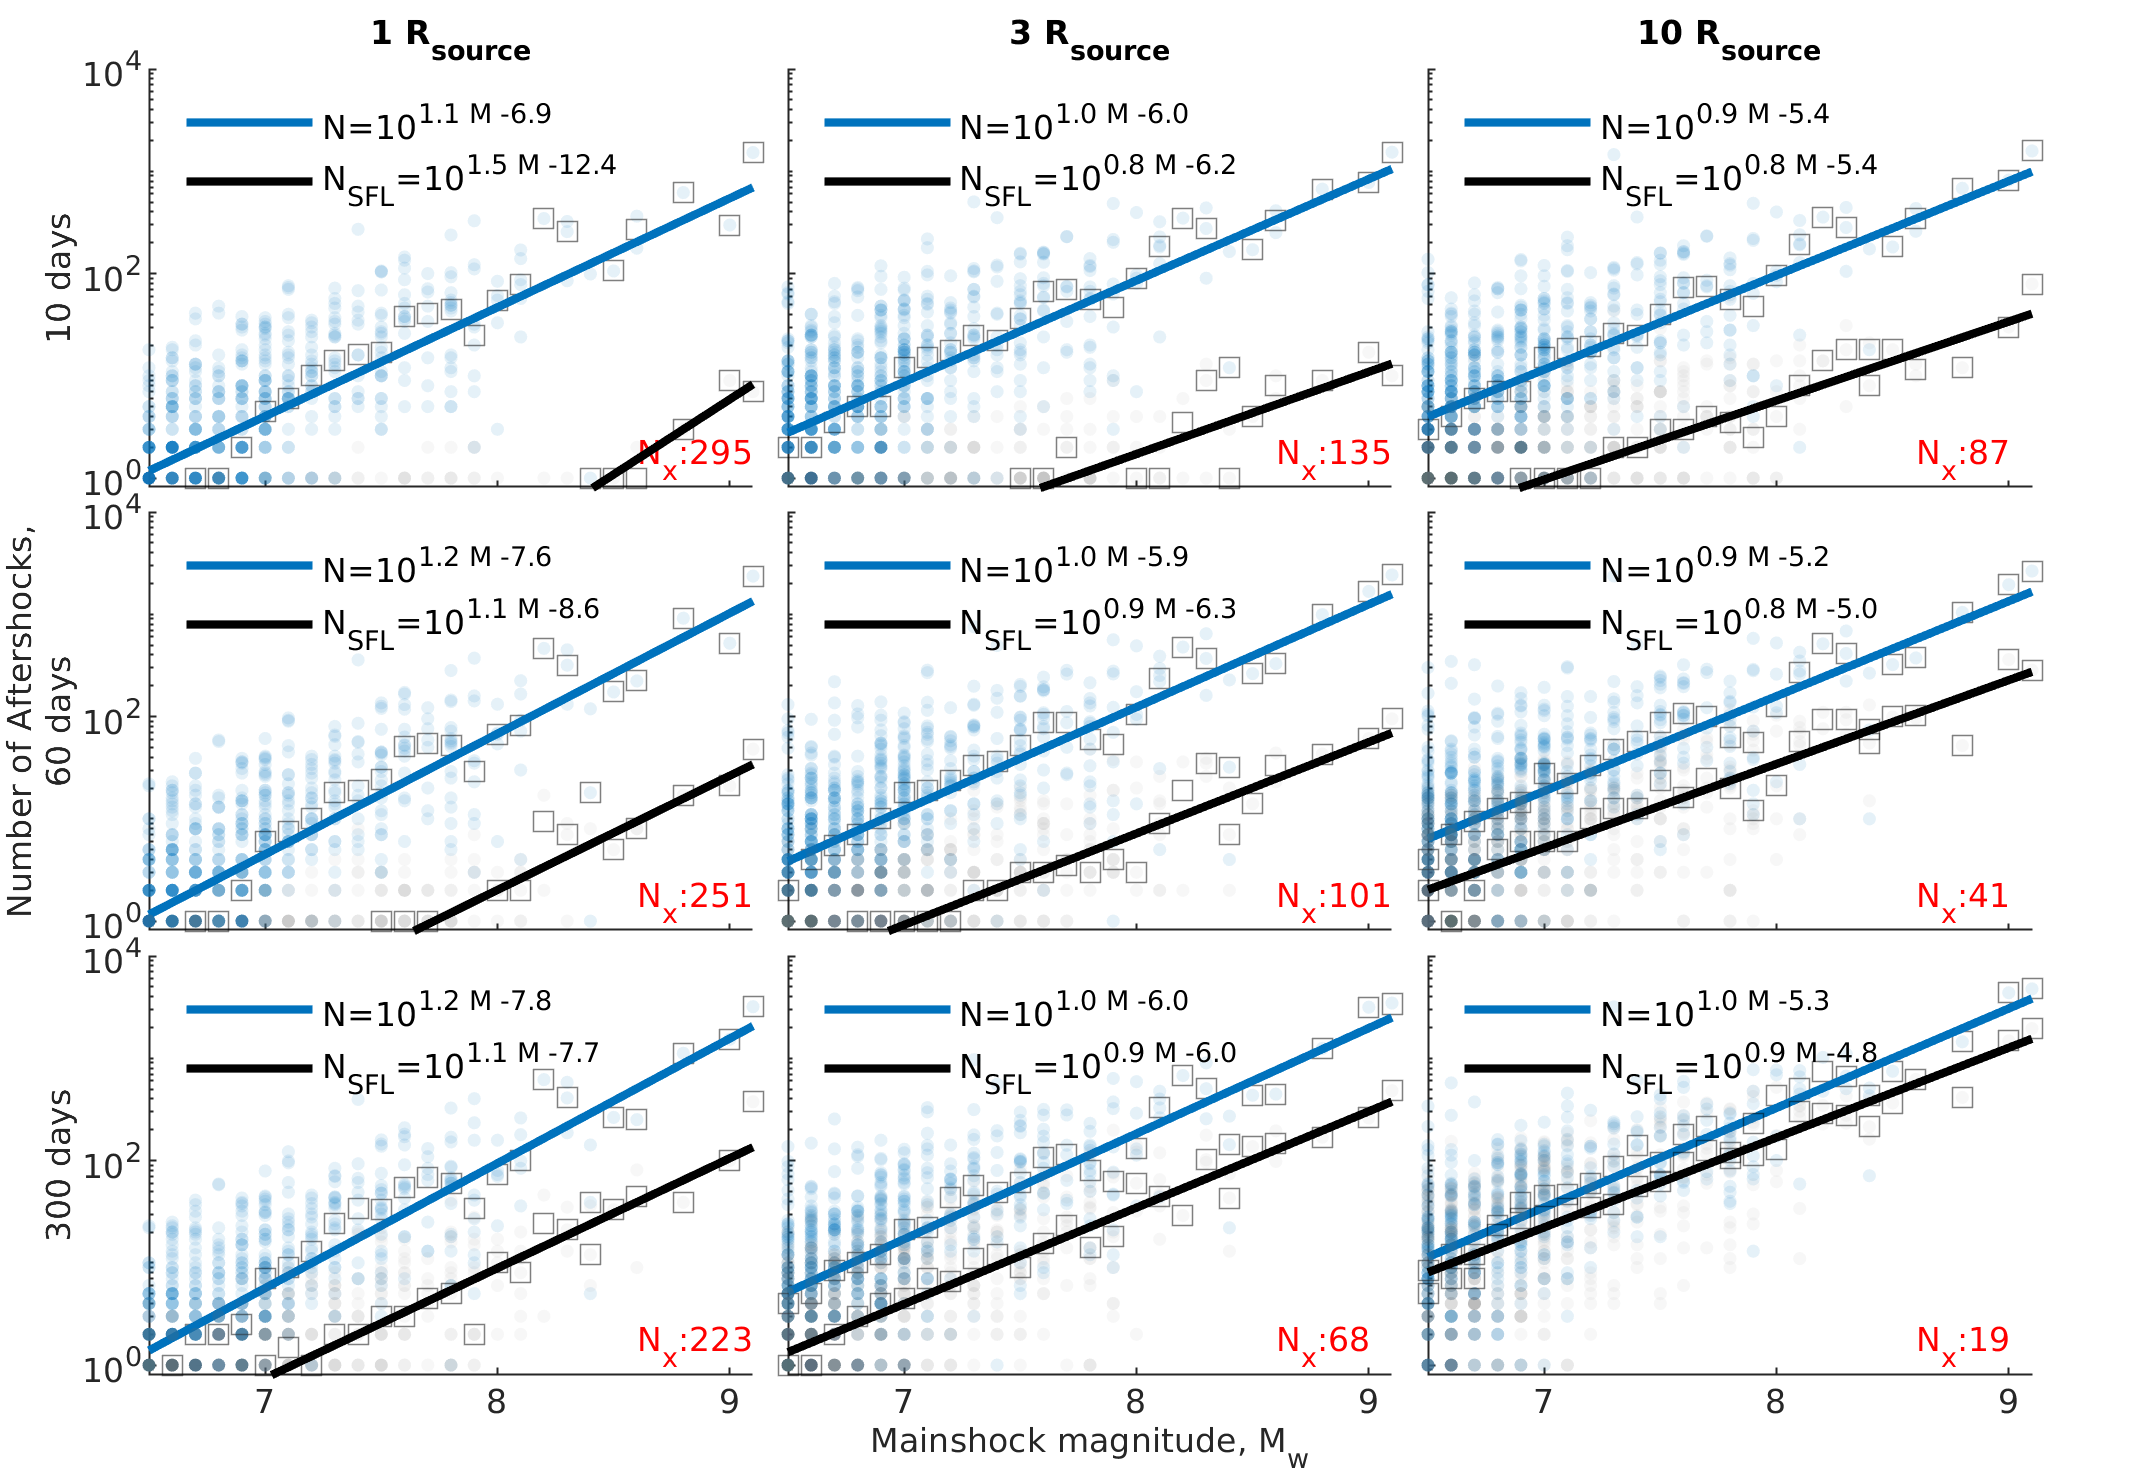
\includegraphics[width = \textwidth]{sensitivity.png}
    \caption{Sensitivity analysis of space-time windows. Time windows of 10, 60, and 100 days and spherical space windows with radii of 1, 3, and 10 source dimensions ($R_{source}$) are considered. \add{Corresponding larger space and time windows are $4/3$ and $5/3$ of the selection windows}. Blue circles are individual mainshocks identified with the hierarchical counting routine. The blue line indicates the outcome of a regression of the median log-number of aftershocks for each 0.1 magnitude bin (blue squares). For reference, we computed the same productivity relationship, $N_{SFL}$ (black line), for the median of 100 time-shuffled catalogs (grey squares). For each space-time window, we indicate the number of mainshocks with no aftershocks in red ($N_x$). Note that as space and time windows increase, more mainshocks have measurable aftershock counts. \change {However, the likelihood of counting background productivity and significantly affecting subsequent parameterization becomes an increasing concern}{However, with increasing time and space windows background events inflating aftershock counts and reducing $\alpha$-values by overestimating the productivity of smaller events becomes increasingly prevalent.}
}
    \label{fig:sensitivity}
\end{figure}


\add{For our alternative method, we use a clustering routine} \citep[following][]{Zaliapin2008, Goebel2019AftershockOklahoma}. \add{This approach seeks to build earthquake families by linking earthquakes to parent events based on a distance metric that combines magnitude, space and time. Pairs of parent and daughter events exhibit a statistical distribution with two modes: one that corresponds to clustered events and another that arises from a Poissonian background of seismicity. Separation of earthquake clusters is achieved by defining a decision boundary between these two modes and cutting all links that exceed this threshold. The largest event in each cluster is identified as a mainshock and aftershocks are counted as the number of events that follow it. See} \citet{Zaliapin2008} \add{for a detailed overview of the method, distance metrics, and theoretical connections to other schemes (ETAS). The specific parameters selected are consistent with previous implementations of} \cite{Zaliapin2008} \add{and are documented fully in the supplementary material (supplement Section S3.3). Supplement figure S16 shows that the aftershock productivity measured from both methods correlate well ($R^2=0.96$). This consistency stems from the relatively high completeness of our catalog which ensures that, for the relatively short time intervals of our aftershock windows, few, if any, background events are likely to be included in the event counts.}

\add{For both methods,} we next compute the median number of aftershocks for each 0.1 magnitude bin in the mainshock catalog (including the counts of events with zero aftershocks) and the corresponding magnitude bin to perform a linear least squares inversion to determine $k$ and $\alpha$ (Figure \ref{fig:fms_prod}a). Using these parameters, we define the relative productivity ($\Delta \log(N)$) for each mainshock as
%
\begin{linenomath*}
\begin{equation}
    \Delta \log(N) = log(N) - log(\hat{N}(M)) = log\left(\dfrac{N}{k10^{\alpha M}}\right)
    \label{eq:residual_productivity}
\end{equation}
\end{linenomath*}
%
where $N$ is the number of aftershocks following a mainshock and $\hat{N}(M)$ is the number of aftershocks predicted for the mainshock magnitude, $M$, from Equation \ref{eq:productivity}.

\add{The relative productivity is closely related to variations in the Omori $a$-value or $K$ value} \citep[e.g.][]{Page, Hardebeck2018UpdatedParameters, Utsu1995,Ogata1988}. The use of \add{$\Delta \log(N)$ as a measure of relative productivity provides a means to assess whether scatter in aftershock production is related to specific mainshock parameters on an earthquake by earthquake basis}.

\add{It is important that relative productivity be independent of magnitude, as we run the risk of confounding variations in the average size of earthquakes with variations in productivity. We show that the median and interquartile range of relative productivity are not magnitude-dependent} (Figure \ref{fig:fms_prod}b \add{and Supplement Figure S1). Note that median and interquartile statistics which we use throughout ensure that we account for earthquakes with no aftershocks which have $\Delta \log(N) = -\infty$.}

\section{Results}
    \subsection{The Global Earthquake Productivity Map}\label{sec:glob}

    Our analysis yields 1011 earthquake sequences with mainshocks exceeding $M_W>6.5$. We map the global catalog of aftershock productivity (Figure \ref{fig:global_res}). We highlight characteristic global patterns which we will examine in more detail in the following sections.

    \begin{figure}
    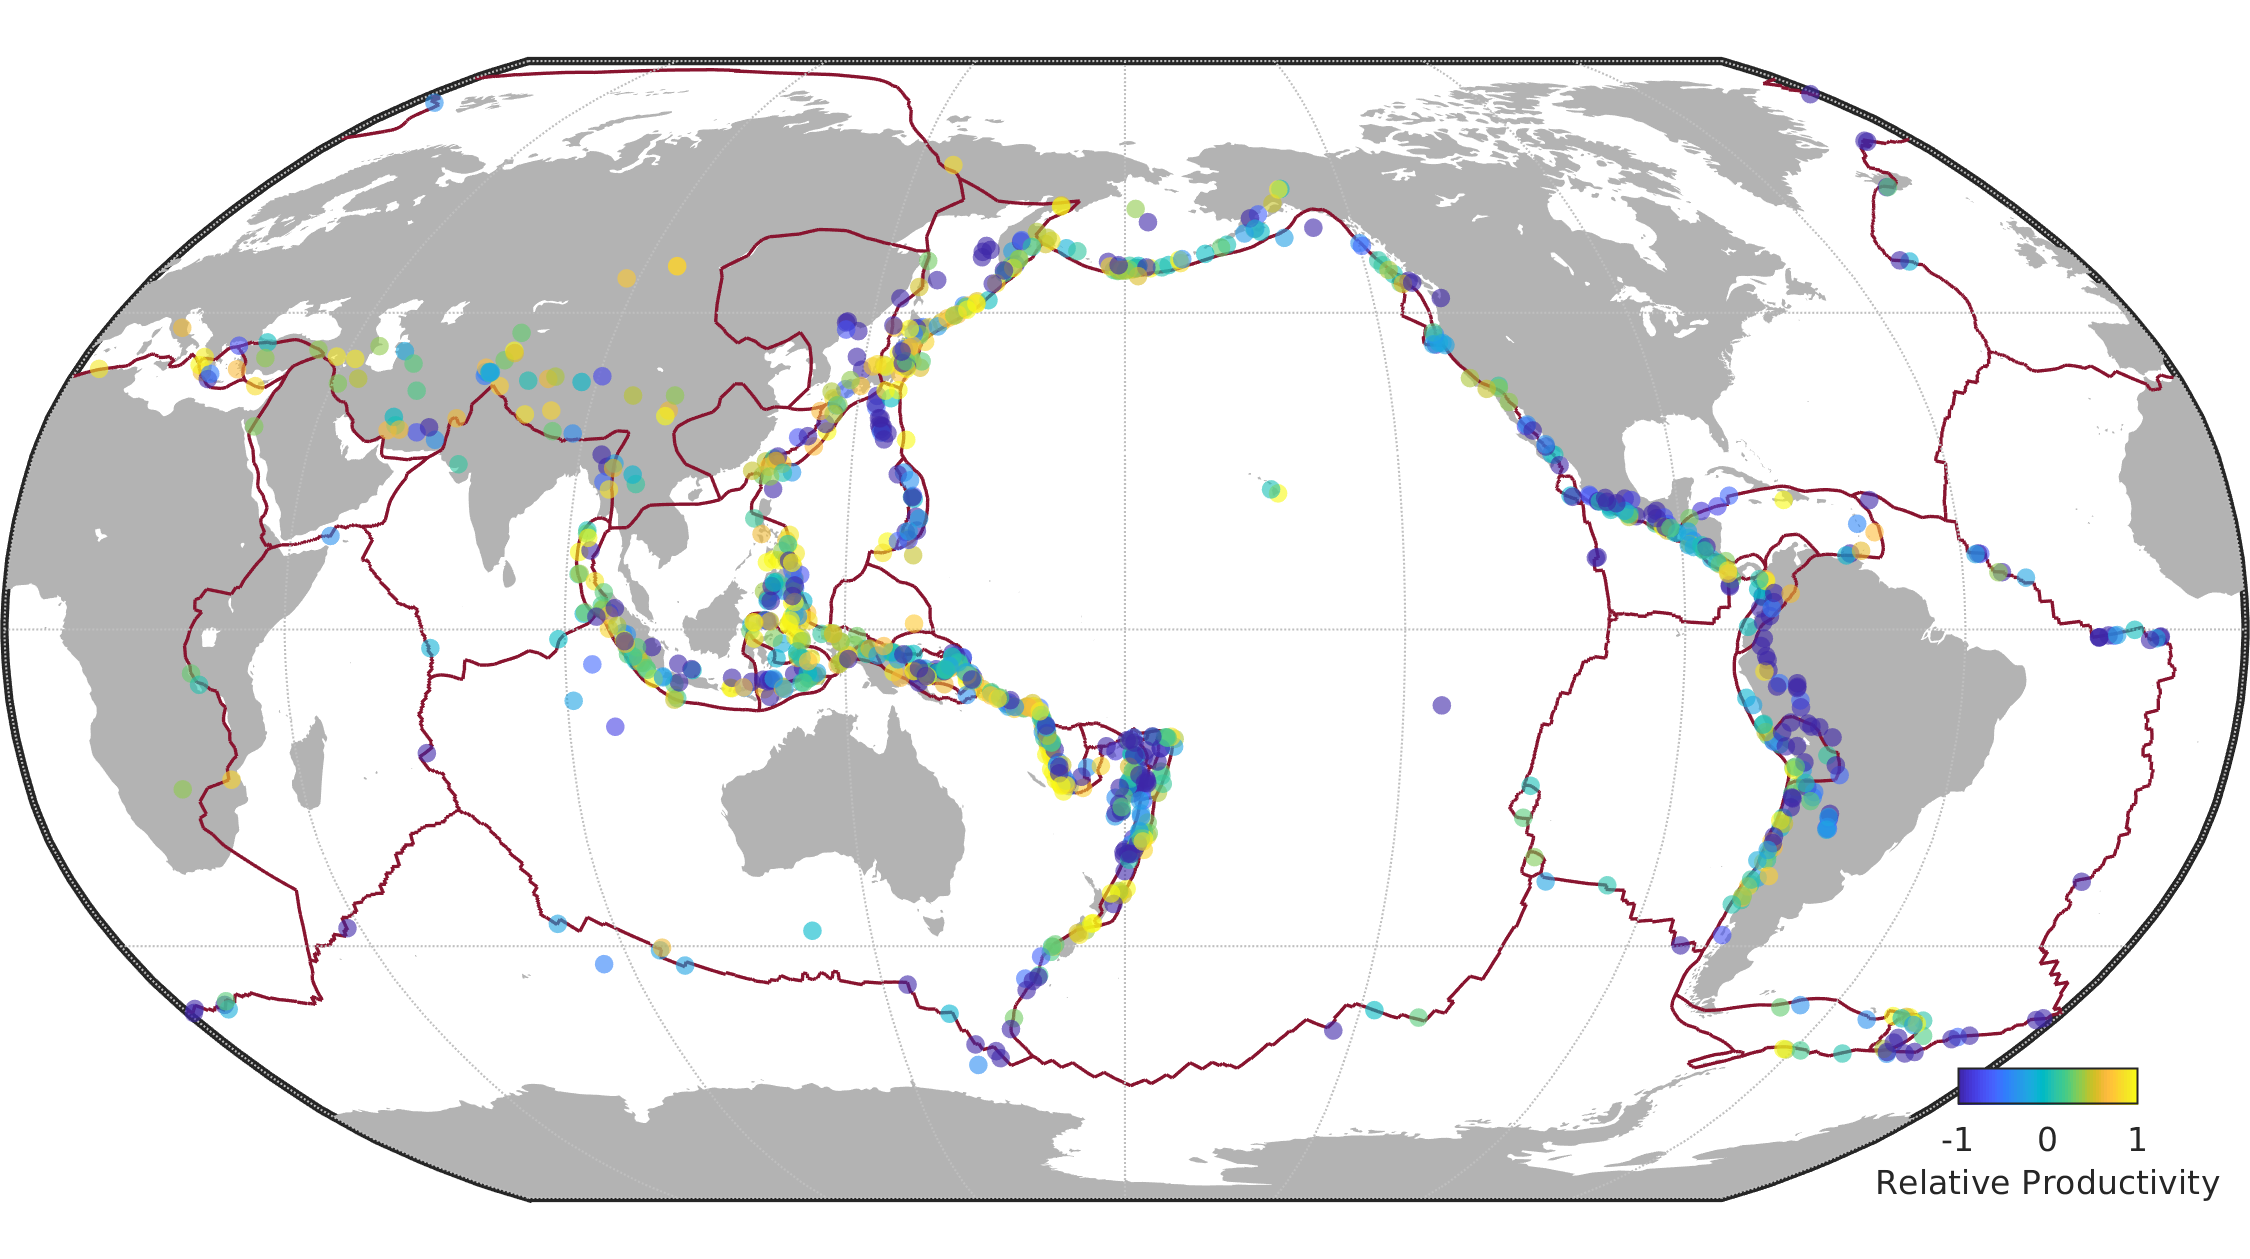
\includegraphics[width = \linewidth]{worldmap_res.png}
        \caption{Global map of earthquake productivity. Red lines indicate the surface trace of the tectonic boundaries. Mainshocks with $M_W\ge6.5$ color-coded according to their relative productivity (Equation \ref{eq:residual_productivity}).
        }
        \label{fig:global_res}
    \end{figure}

    Intermediate- and deep-focus earthquakes stand out in the relative productivity map. Continental-scale bands of earthquakes with low relative productivity run along the Atacama, Japan, Izu-Ogasawara, Mariana and Tonga trenches. These are predominantly normal and reverse earthquakes rupturing intermediate- to deep-focus seismic zones. Over the entire catalog, earthquakes deeper than $\sim55$~km exhibit decreasing relative productivity with increasing depth (Figure \ref{fig:prod_vs_depth}). Similar observations are well documented \citep{Bath1965LateralMantle, Frohlich1989TheEarthquakes, Nyffenegger2000, Wiens1997AftershockZone, Wu1999, Houston2004}. We, therefore, do not include mainshocks deeper than 55~km  in the following analysis to avoid confounding depth with other influences.

    \begin{figure}
        \centering
        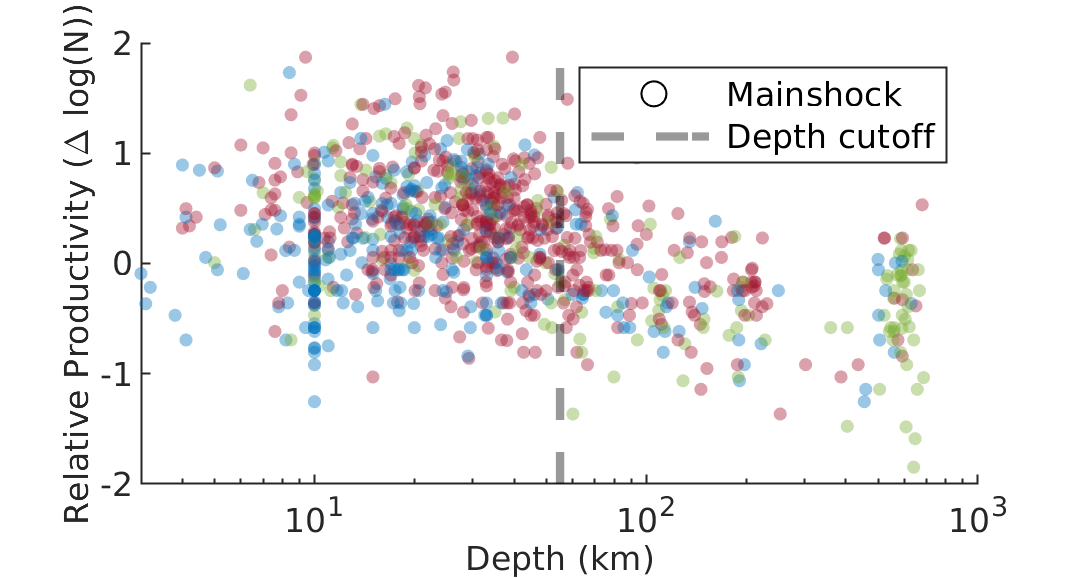
\includegraphics{prod_vs_depth.png}
        \caption{Relative aftershock productivity as a function of depth. Subsequent analysis will only consider earthquakes shallower than the 55~km cutoff (dashed line). Sequences are color-coded according to faulting style of the mainshock (blue: strike-slip, green: normal and red: reverse).\add{Note: Discretization of depth is apparent in this plot as some events have default values. Depths of  33~km, 5~km, 10~km and 15~km are reported for  6\%, 1\%, 10\% and 0.7\%, respectively, of the catalog.}.
        }
        \label{fig:prod_vs_depth}
    \end{figure}

    Offshore earthquakes that are not in subduction zones have lower relative productivity. Oceanic transform and divergent boundaries usually host less productive aftershock seismicity than the global trend ($\Delta \log(N)<0$). Consider for example the 2018 $M_W7.5$ earthquake north of Honduras rupturing the Swan Islands oceanic transform fault. It had 2 aftershocks with $M_W>4.5$ within 150 km of the epicentral location; for reference, the global median aftershocks count for mainshocks of $M_W7.5$ is 11 and therefore $\Delta log(N) = -0.7$. Earlier earthquakes along the transform have similarly low relative productivity. There are very few of these offshore events that are productive. \add{With 170 aftershocks within 792 km,} the $M_W8.6$ 2012 intraplate strike-slip rupture offshore Sumatra followed by a $M_W8.2$ aftershock appears to be among the most productive earthquakes hosted in oceanic lithosphere not within a convergent boundary ($\Delta log(N) = -0.15$).

    The western coastline of North America hosts spatially coherent patterns in relative aftershock productivity (Figure \ref{fig:region}a). The Aleutian Arc grades from earthquakes with generally high aftershock productivity in the West to low aftershock productivity in the East. Earthquakes on the Queen Charlotte Fault exhibit aftershock abundances similar to the global average. Offshore clusters of seismicity along the Blanco Fracture Zone and the Mendocino Triple Junction have low productivity. Continental earthquakes along the San Andreas Fault System are markedly more productive than the seismicity to the north and south. The pronounced decrease in productivity at the southern terminus corresponds to a shift from generally transpressional continental- to transtensional oceanic-tectonics. Subduction of the northernmost section of the Cocos plate under Mexico is associated with low aftershock productivity. The number of aftershocks increases southward along central America. The gradational increases in productivity along the Aleutian Arc (westward) and Cocos Subduction zone (northward) correspond to increasing lithospheric age of the oceanic plate (Figure \ref{fig:region}b).

    \begin{figure}
        \centering
        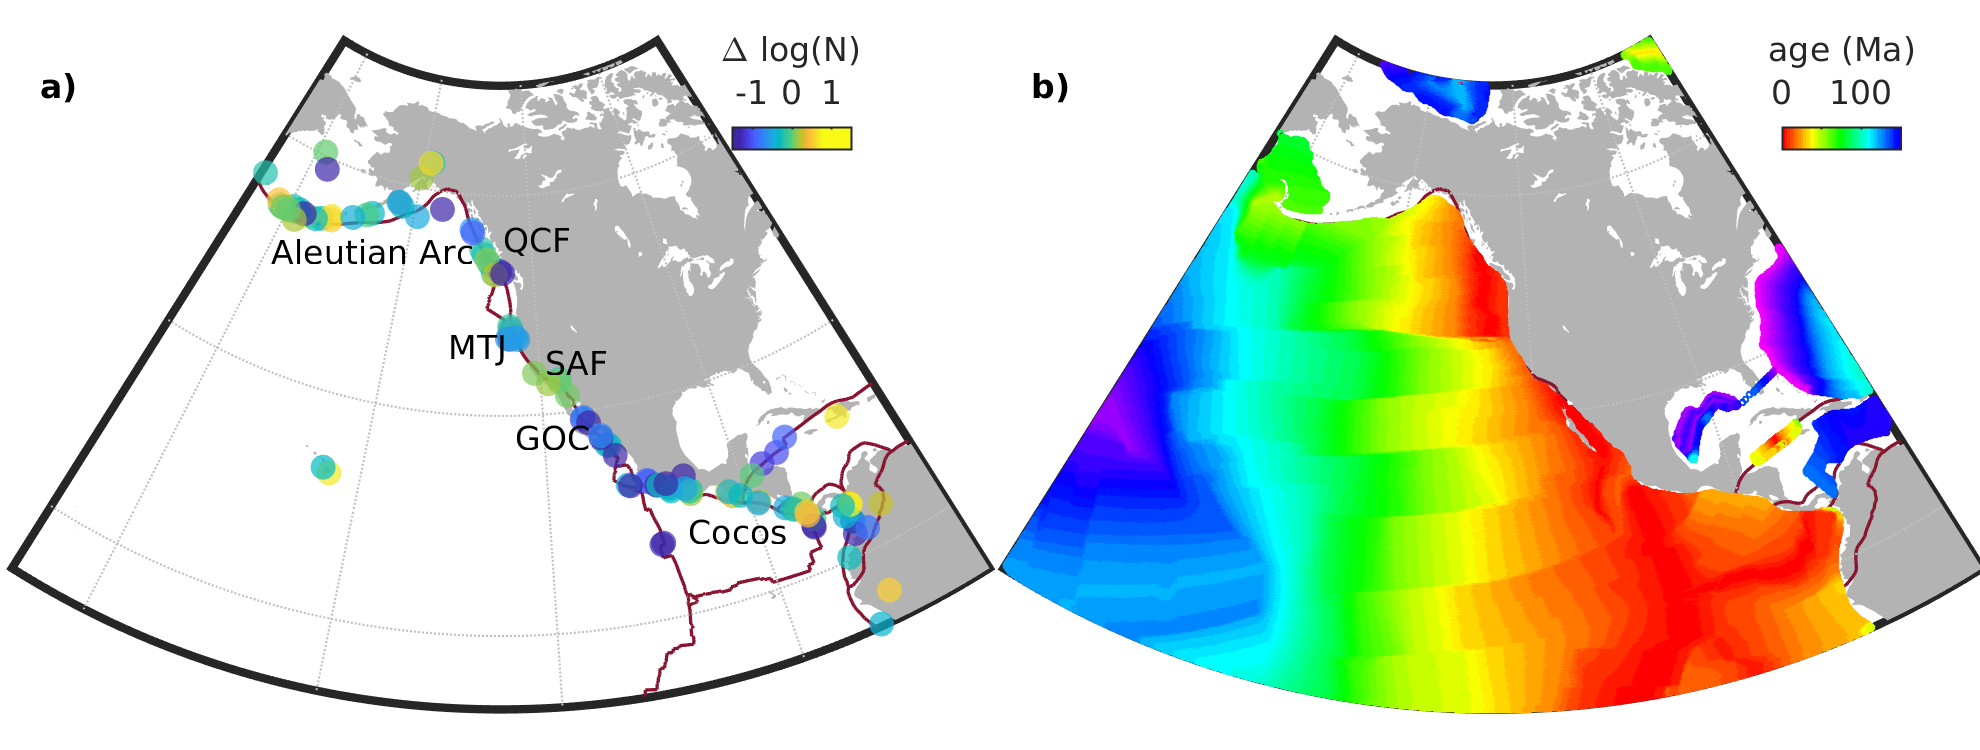
\includegraphics[width = \linewidth]{regions.png}
        \caption{a) Aftershock productivity along the North American coastline.  Individual mainshocks (circles) are color-coded according to their relative aftershock productivity ($\Delta \log(N)$, Equation \ref{eq:residual_productivity}). The Aleutian Arc, Queen Charlotte Fault (QCF), Mendocino Triple Junction (MTJ), San Andreas Fault (SAF), Gulf of California (GOC) and Cocos Plate Subduction Zone include areas with coherent productivity. Red line indicates major plate boundaries \citep{Bird2003AnBoundaries}. b) Seafloor crustal age estimates from \citet{Muller2008}.}
        \label{fig:region}
    \end{figure}

    Continental seismicity has elevated aftershock productivity. Most notable is the India-Asia Collision Belt. Other examples include onshore seismicity in New-Zealand, the San Andreas Fault, and the Arabian Plate collision.

    \subsection{Tectonic Setting Effects}\label{sec:tectonic_setting}

    We investigate the effect of the seismo-tectonic setting on the productivity of earthquake sequences. Specifically, we subdivide the mainshock catalog by plate boundary following the categorization detailed in Table \ref{tbl:attributes}. This comparison is shown in Figure \ref{fig:plate_boundary}. The results single out oceanic transform faults as particularly deficient in aftershocks. Continental transform faults, are more productive, but less so than the global average. Subduction zones, continental convergent boundaries, continental rift basins, and oceanic convergent boundaries have similar and generally elevated relative productivity. A \add{two-sample} Kolmogorov\-Smirnov test \add{comparing the cumulative distribution of each subset to the entire set} suggests that the relative productivity of events on oceanic transform faults and continental convergent boundaries have small probabilities, $1/10^9$ and $3/10^4$ respectively, of being randomly sampled from the overall distribution by chance; the remainder of the subsets are not significantly different from the overall distribution ($p = 0.05$ or, equivalently, a  $1/20$ chance).

    \begin{figure}
        \centering
        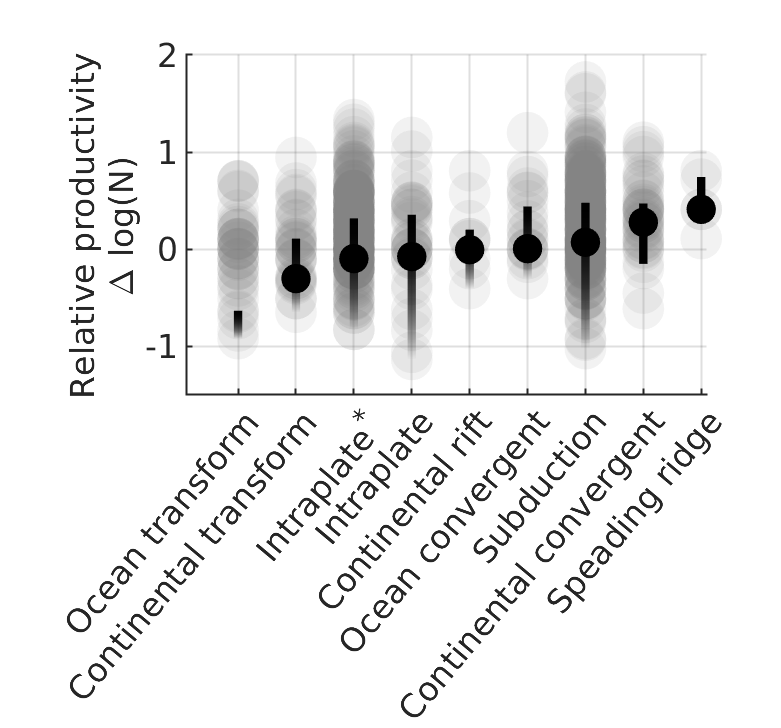
\includegraphics{prod_by_pb.png}
        \caption{Earthquake productivity by tectonic boundary. Circles indicate the relative productivity of individual sequences. Solid markers and error bars indicate the median and the interquartile range. A faded lower error bar implies that mainshocks with no aftershocks are within the interquartile range. Intraplate$^*$ indicates earthquakes within 400 km of a plate boundary but with a faulting mechanism discordant with the plate boundary (e.g., outer rise events).}
        \label{fig:plate_boundary}
    \end{figure}

    Earthquake productivity is also related to the age of the lithosphere  (Figure \ref{fig:prod_vs_age}). Earthquake sequences in younger oceanic lithosphere tend to have fewer aftershocks. Considering all mainshocks, we observe a more systematic increase in median productivity for earthquake sequences in oceanic lithosphere less $\sim 40$ Ma in age. Strike-slip mainshocks best define the trend. Consistent with the trend, earthquakes with no aftershocks are strongly biased to oceanic lithosphere with young ages; within $<$40 Ma oceanic lithosphere, the fraction of mainshocks with no aftershocks is approximately twice the global average. Performing the same analysis using a more conservative magnitude of completeness of $M_W5$ yields the same behavior, thus ensuring that the trend is not an artifact of instrumentation and catalog completeness (supplement Figure S11).

    \begin{figure}
        \centering
        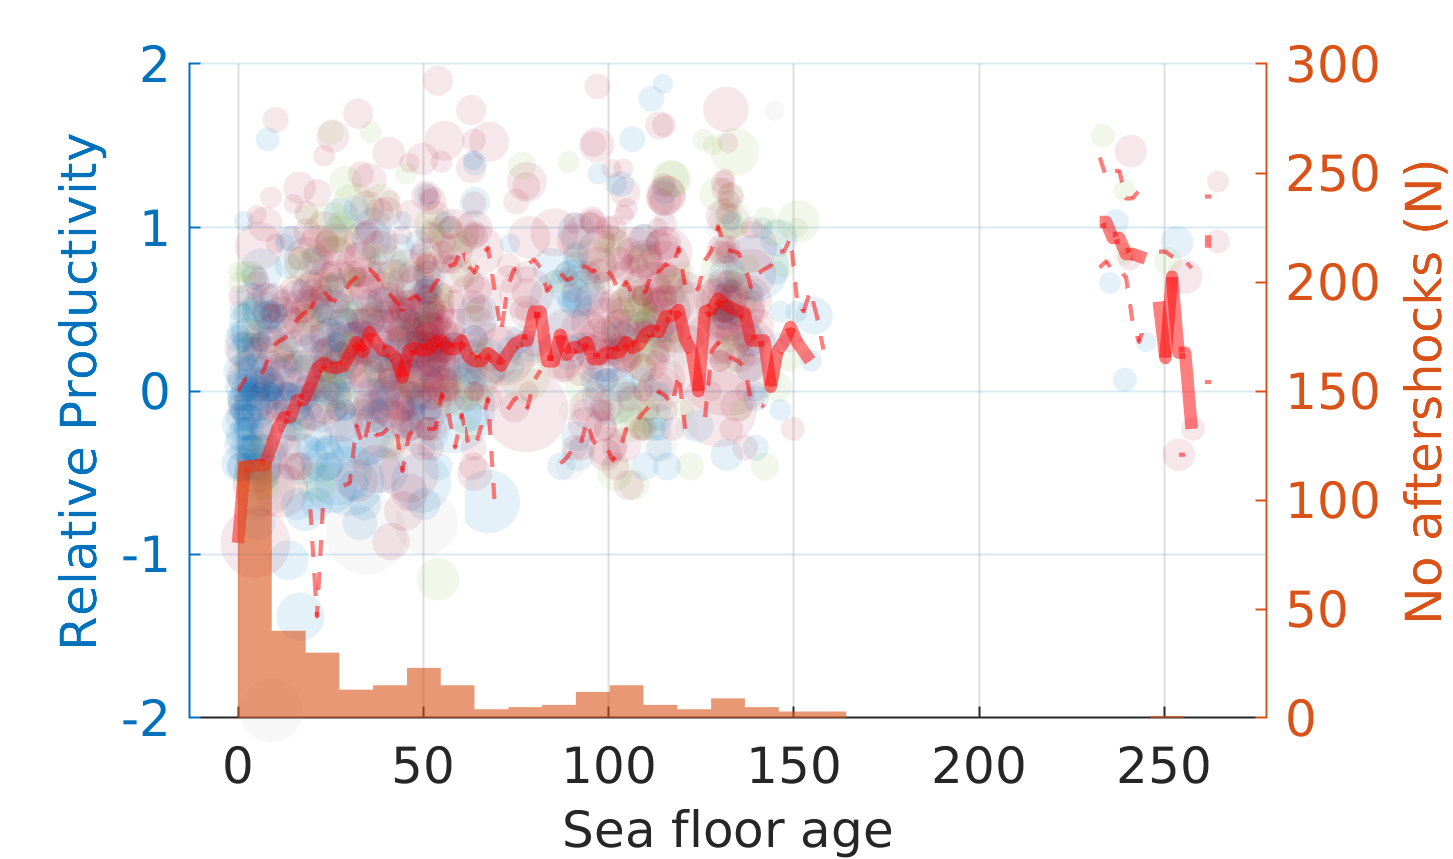
\includegraphics{prod_vs_age.png}
        \caption{Relative productivity increases as a function of the age of the oceanic lithosphere. Each circle indicates an individual earthquake sequence. Sequences are color-coded by faulting style of the mainshock (blue: strike-slip, green: normal and red: reverse). The red line indicates the median average for 20~Ma crustal age bins. Dashed lines indicate the corresponding interquartile ranges. Vertical grey bars indicate the fraction of earthquakes with no aftershocks within each 10Ma crustal age bin \add{and correspond to the right-hand axis}.}
        \label{fig:prod_vs_age}
    \end{figure}

    \subsection{Source Effects}\label{sec:source_parameters}

    To identify mainshock source effects that may influence relative aftershock productivity, we linearly regress each available parameter with the relative productivity and compare the goodness of fit to random trials. The variance reduction for each regression is presented in Figure \ref{fig:r2_finite_fault}a.

    At face value, this analysis shows that aspect ratio, width, and stress drop are best correlated with the relative productivity. Figures~\ref{fig:r2_finite_fault}b-d show that these correlations are seen in the raw data, albeit with significant scatter.

    \add{A potential problem with this analysis of 12 test parameters is that a spurious correlation could arise simply because of the numerous investigated regressions. We explicitly address this issue by investigating the probability of spurious correlations. To do so, we first remove any causal relationship between our 12 predictors and relative productivity by shuffling the aftershock measurements and randomly reassigning each relative productivity measurement to the parameters for a different mainshock. We then regress each parameter with the relative productivity and report the maximum variance reduction of any parameter in this shuffled set. This same routine is repeated 10000 times to generate a probability distribution function of the maximum variance reduction of 12 parameters should there be no causal relationship in the data.} \remove{To assess statistical significance and guard against spurious correlations, we perform the same regression routine and report the maximum correlation for 10000 random permutations of the catalog with all attributes under consideration}. We refer to this evaluation of the extreme value for the full group, or family, of parameters as a family-wise test and it serves as a \remove{robust and conservative} null hypothesis. \add{We determine the percentile of our actual regression results within these random realizations, the family-wise p-value, for comparison} (Figure \ref{fig:r2_finite_fault}a - top axis). \remove{Comparing our results to the shuffled realizations of the data} The comparison yields the probability of obtaining equally good or better results by chance.

    The rupture's normalized energy, normalized length, normalized area, Poisson's Ratio, log-heterogeneity, Young's Modulus, and velocity all yield \add{a variance reduction with more than a 1/20 chance to arise by chance for the shuffled data and are thus not further considered.} Refer to the supplement (Figure S12) to see all correlations \citep{Convers2011GlobalMid2010, Hayes2017}.

    \remove{Our analysis suggests that correlations with log-stress drop and normalized width are mar\-gi\-nally significant. Slip-zone aspect ratio is related to relative productivity in a statistically significant sense. Aftershock productivity negatively correlates with the logarithm of stress drop and aspect ratio, and positively correlates with normalized rupture width (see Figure b-d).}

    \add{Our analysis suggests that correlations with log-stress drop ($p = 0.07$) and normalized width ($p = 0.05$) are mar\-gi\-nally significant. Aftershock productivity negatively correlates with the logarithm of stress drop and positively correlates with normalized rupture width} (see Figure \ref{fig:r2_finite_fault}b-c)

    \add{Slip-zone aspect ratio ($p = 0.007$) is related to relative productivity in a statistically significant sense. Aftershock productivity negatively correlates with aspect ratio} (see Figure \ref{fig:r2_finite_fault}d).

    \begin{figure}
        \centering
        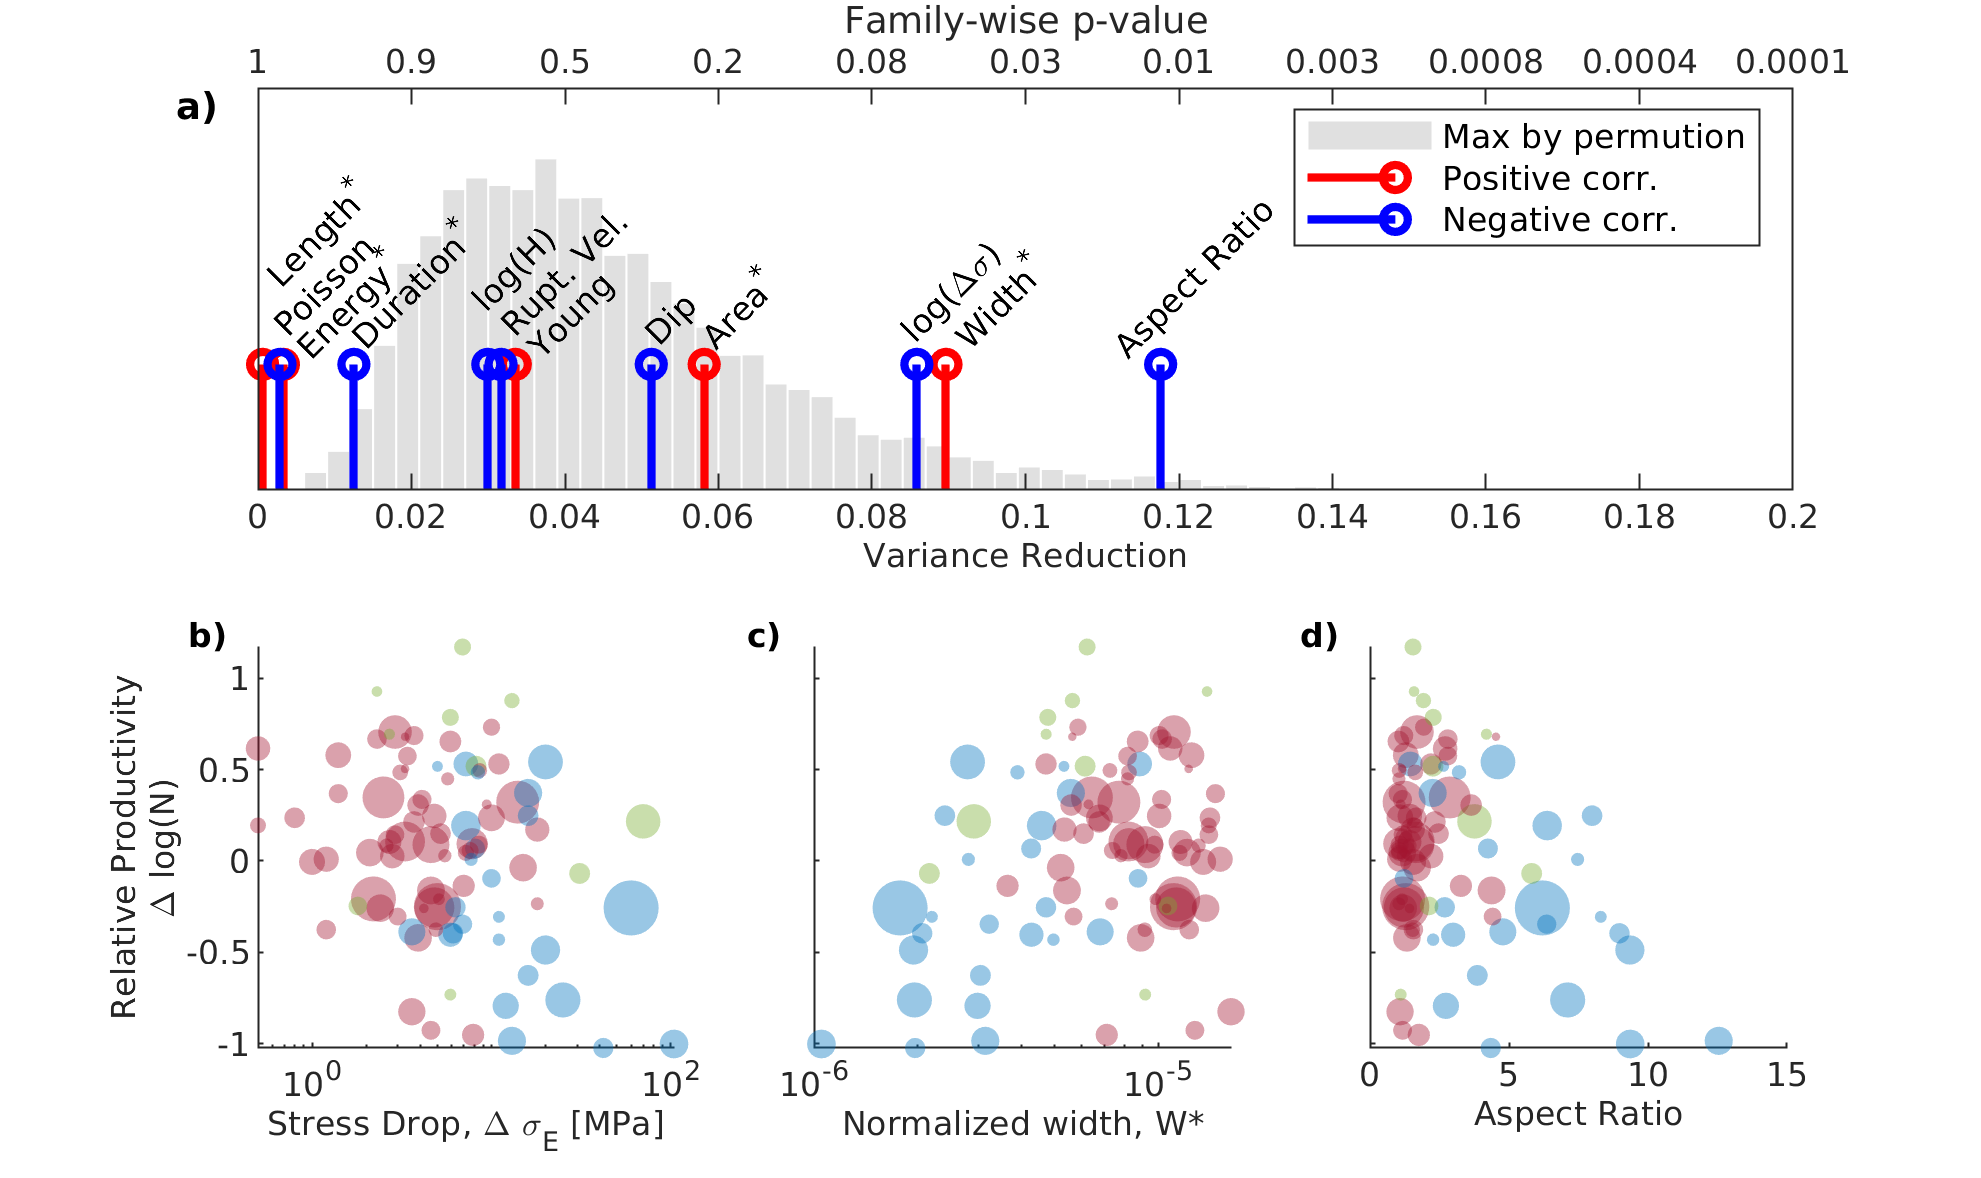
\includegraphics[width = \linewidth]{stem_plot.png}
        \caption{a) Goodness of fit of linear regressions for each source attribute in our combined catalog. Top and bottom axes respectively represent the p-value and goodness of fit of each attribute (stems). The probability distribution function in the backdrop indicates the maximal variance reduction outcome of 10000 permutation test of the entire data set. Asterisks indicate scaled and log-transformed variables. The scaled energy, length, duration and area, material properties, velocity, dip, and log-stress drop ($\Delta\sigma$) of the mainshock rupture all do not yield a statistically significant ($p=0.05$) linear fit to the relative productivity — the normalized rupture width and aspect ratio of the rupture yield the best fitting linear regressions. Stems are color-coded to indicate whether the source attribute is positively (red) or negatively (blue) correlated with relative productivity. b-d): Relative earthquake productivity as a function of mainshock stress drop, normalized rupture width, and aspect ratio. Individual mainshocks are color-coded according to faulting style as in Figure \ref{fig:fms_prod}.}
        \label{fig:r2_finite_fault}
    \end{figure}

    \subsection{Focal Mechanism Dependence of Aftershock Productivity}

    Aftershock productivity exhibits a strong relationship with focal mechanism of the mainshock (Figure \ref{fig:coloc}a). Strike-slip mainshocks have relatively few aftershocks. The median number of aftershocks for strike-slip mainshock is three times fewer than dip-slip mainshocks of comparable magnitude. This separation by focal mechanism far exceeds 95\% confidence intervals ($p\ll 0.05$).

    Whether this is a site or source effect is ambiguous. To further investigate this question, we examined whether earthquakes with different focal mechanisms that share the same geographic location still exhibit statistically distinct earthquake productivity. If the tectonic setting is the only control on the relative productivity of earthquakes, then strike-slip earthquakes should not have fewer aftershocks when controlling for location.

    We construct a catalog of co-located strike-slip and dip-slip earthquake pairs by iteratively cataloging the nearest pairs of strike-slip and dip-slip mainshocks. We explicitly avoid double counting throughout this process and ensure regular global coverage. The productivity of co-located strike-slip and dip-slip earthquakes generally follows a 1:1 trend (Figure \ref{fig:coloc}). The distinction by faulting style is not statistically significant when comparing only co-located earthquakes ($p = 0.63$). This shift indicates that event-location alone partially explain why strike-slip earthquakes are deficient in aftershocks. Significant scatter implies that source effects (e.g., aspect ratio, stress drop, and dip) may contribute to the distinction.

    \begin{figure}
        \centering
        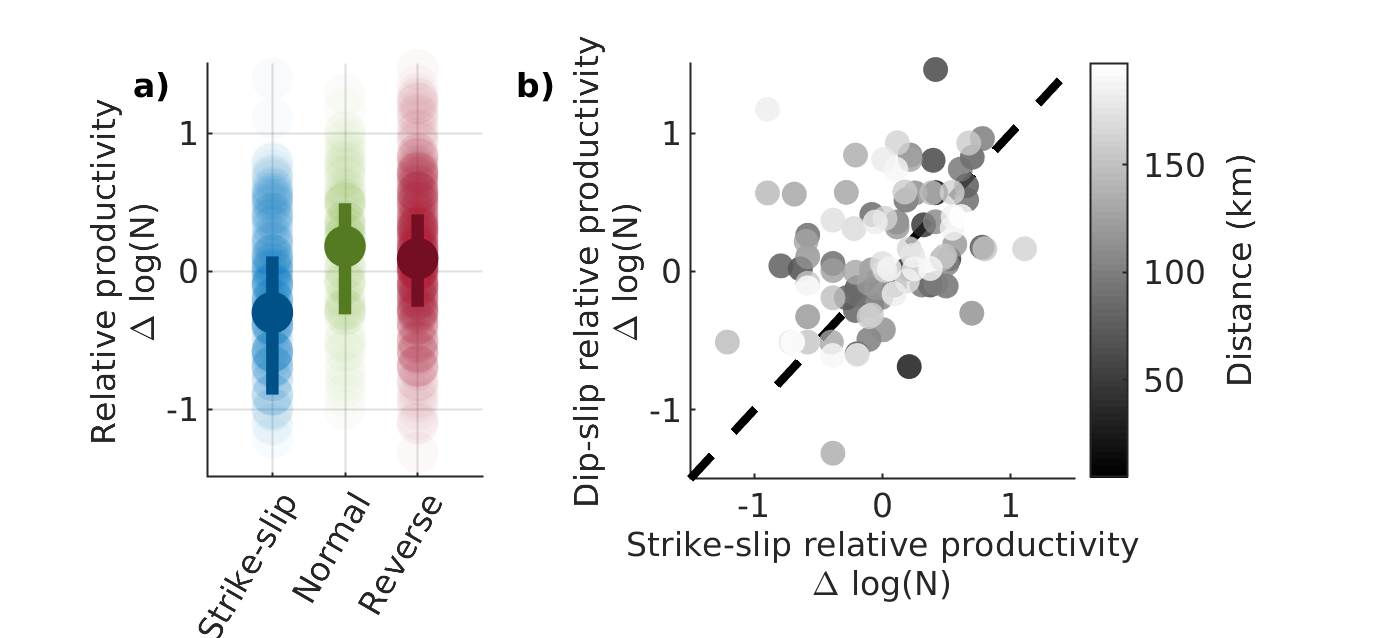
\includegraphics{fmspairs.png}
        \caption{a) Relative aftershock productivity, $\Delta \log(N)$, by focal mechanism (Equation \ref{eq:residual_productivity}). b) Relative aftershock productivity for pairs of earthquake sequences with strike-slip and dip-slip mainshocks within 200 km from each other. Each pair is shaded according to its relative distance. Dashed line indicates a 1:1 relationship, the expectation for a purely site dominated control on relative productivity. Co-located mainshocks pairs generally follow this 1:1 trend, but exhibit considerable scatter.}
        \label{fig:coloc}
    \end{figure}

    \subsection{A Multi-Attribute Prediction of Aftershock Productivity}

    We have considered variables on a case by case basis and have prescribed a functional form to the relationships. In this section, we allow for increased complexity by utilizing machine learning tools to predict relative productivity given contextual information about the mainshocks setting and kinematics. \add{We measure the performance of these tools by computing the root mean squared value,} $RMSE = \sqrt{\dfrac{\sum{(\hat{f_i}-f_i)^2}}{N}} $, where $\hat{f_i}$ \add{is the prediction of relative productivity and $f_i$ are one of $N$ observed values}. \add{To avoid over-fitting the data, we perform leave-one-out cross-validation---individual predictions are calibrated on the remainder of the data} \citep{witten2011}.

    As a point of reference, we produce predictions of relative productivity based on local seismicity. In this approach, aftershock productivity is predicted based on the median relative productivity of the 50 nearest mainshocks. Prediction accuracy is largely insensitive to the number of neighbors (20-100 yield comparable results). The chosen number of nearest neighbors produces the \change{best predictions}{lower root mean squared error between predictions and observed relative productivity measurements}. Model validation is shown in Figure \ref{fig:response}a. This approach captures geographical effects, provides a 8\% forecast improvement in the RMSE when compared to the global productivity law, and serves as a baseline for the following.

    We then tabulate earthquakes for which all parameters exist and systematically test predictions based on permutations of parameters on various machine learning algorithms. \remove{To avoid over-fitting the data, we perform leave-one-out cross-validation---individual predictions are calibrated on the remainder of the data} Support Vector Machines (SVM) yield the \change{best predictions}{lowest root mean squared error} (Figure \ref{fig:response}b). Support vector machines aim to find lines, planes, or hyperplanes, that minimize the error of the data by mapping data to higher dimensional spaces with transformations called kernels. \add{Key differences between SVM regression and a typical linear regression are 1) a tolerance for a margin of error, 2) an explicit minimization of model complexity using a  penalty for each additional input parameter and 3) an embedded non-linearity enabled by the transformation of the coordinate system via prescribed kernel functions. Required model hyperparameters are the order of the kernel polynomial transformation, the margin width, and the complexity trade-off.} SVMs are robust to over-fitting data and are therefore well suited for small datasets \citep{witten2011}. \add{We present results from an SVM model trained using a quadratic kernel. The trained model is included in the supplemental files with full documentation of hyperparameters.}

    The following metrics yield the best predictions of relative productivity: scaled rupture area, fault dip, and plate age. Better predictions on training data, with adverse predictions on the validation data, indicate that additional parameters do not improve predictions and instead induce over-fitting.

    The root mean squared error of the final model predictions of the SVM is 0.40, a 27\% improvement on the global productivity law and a 20\% improvement on the nearest neighbor algorithm, despite employing no direct geographical information. Notably, the SVM model better predicts extreme cases (highly productive or unproductive). The root mean squared error of the SVM is influenced by the following two outliers, the 2017 $M_W7.0$ Loyalty Islands earthquake and the 2013 $M_W7.8$ Scotia Sea earthquake. The productivity of these events is underestimated by the model. Interestingly, both these mainshocks were preceded large foreshocks: two $M_W6+$ earthquakes for the former and a $M_W6.8$ earthquake for the latter. Removing these two outliers yields an additional 10\% improvement to the predictions.

    \begin{figure}
        \centering
        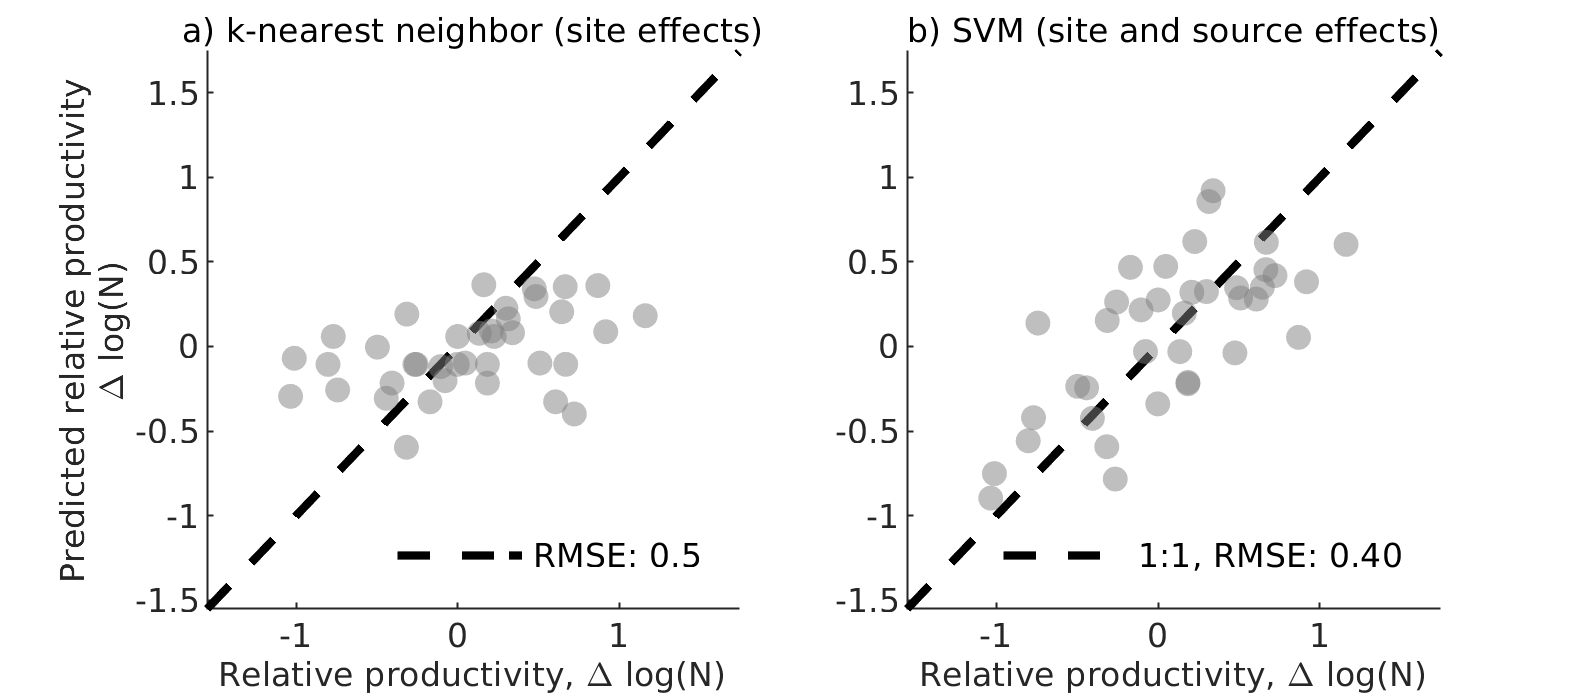
\includegraphics{response.png}
        \caption{Response plots (prediction versus observation) for the k-nearest neighbor algorithm (a) and SVM models (b). Each point indicates prediction of relative productivity relative to that which was observed for individual earthquake sequences. A perfect prediction would place all values on the 1:1 line. \add{The SVM model provides a 22\% improvement in the root mean squared error when compared to} k-nearest neighbor model. Combining both contextual information about the setting (crustal age) and the source (dip and normalized area) yields a root mean square value of 0.40.}
        \label{fig:response}
    \end{figure}

The preferred parameters of the SVM can be compared to those found in section \ref{sec:source_parameters}. For instance, dip appears to be more important in the SVM case. Aftershock productivity relates to dip non-monotonically with a maximum at intermediate  dips ($\sim 25^o$) (See Figure S12, Panel l). The added non-linearity allowed by the SVM model kernels is useful in this situation. Normalized rupture area is also more important in the SVM than in the linear regressions. This cause of this difference is harder to discern, but is likely a combination of the added non-linearity allowed by the SVM model and the co-variance across the combined attributes. These differences emphasize that the collapse of multivariate data into single attribute linear relationships has its limitations.

 %

  %Redoing Figure~\ref{} with this smaller dataset results in normalized area equivalent variance reduction for both parameters. Intriguingly, the simpler metric that focuses strictly on the geometric extent of the rupture appears to perform better as an aftershock predictor.


\section{Interpretation}

We find that relative productivity is sensitive to both setting and source effects. From setting, dominant factors are lithospheric age, lithosphere type (oceanic vs. continental) and depth; from source, factors are area, width, aspect ratio and stress drop. Focal mechanism is an additional factor that can be construed as stemming from both tectonic setting and source. Figure \ref{fig:caltech} synthesizes these results demonstrating how significant factors compare to each other. \add{Similar results persist from large ($M_W>7.5$) mainshocks to smaller ($6.5<M_W<7.5$) mainshocks, indicating that there is no significant regional scaling differences that confound our results (Supplement Figure S3-4).}

\add{Our results are robust to aftershock selection method and catalog completeness, which are the primary two factors that could influence. A higher catalog completeness of $M_W5$ reproduces similar results to those we presented using a global completeness of $M_W4.5$, though far more mainshocks have no observed aftershocks. When more than half of mainshocks considered in a group are censored, the estimation of a median productivity is obscured. Using an alternative clustering routine, the relationship between relative productivity and crust age is slightly less pronounced but still apparent. Interestingly, we find better relationships between aftershock productivity and normalized rupture area (p=0.004), stress drop (p=0.0008) and normalized width (p=0.002). Note that these changes occurred among variables that are strongly co-varied} (as shown in Figure \ref{fig:covariance}). \add{The correlation between source properties and aftershock productivity are otherwise unchanged using this alternative definition of aftershock clusters. Finally, only subtle changes are incurred when examining our major results} (Figures \ref{fig:caltech} and S25). \add{Consistency with conservative catalog completeness, mainshock size, and aftershock selection method suggest that our major results are robust.}

\subsection{Relative Importance of Setting and Source Effects}

Our parameterization of slip heterogeneity does not correlate well with productivity. This observation contradicts some modelling predictions \citep{Helmstetter2006RelationModel, Marsan2006} and long-standing interpretations \citep{Mogi1967}. The observation suggests that the number of observable aftershocks is dominated by surrounding volume outside the main slip zone and less strongly modulated by residual stress on the fault plane \citep[as would be consistent with][]{Wetzler2018SystematicEarthquakes}. Thus, this particular aspect of source does not appear to exert a strong influence on relative productivity.

Measurements of relative productivity show no correlation with the scaled radiated energy of the mainshock. We gather that within three source dimensions of the mainshock, static and quasi-static effects dominate earthquake triggering.

The relative productivity of high and low stress drop events is weakly separated. High stress drop ruptures drive more elevated stresses at the periphery of the fault which may contribute to higher aftershock productivity; but, this effect is reversed by the size of the rupture fault which is smaller for a high stress drop rupture. Thus, the compactness of the rupture stresses dominates as a smaller volume and triggers fewer aftershocks \citep{Wetzler2016}.


%\citet{Wetzler2016} interpreted higher stress drops to correlate with lower productivity as a result of a geometric effect. Higher stress drop means more compact rupture. Intriguingly, the simpler metric that focuses strictly on the geometric extent of the rupture appears to perform better than stress drop as an aftershock predictor in the SVM model. The normalized rupture area is a more direct measure of this physical relationship.

% Another such competition might occur between elevated aftershock productivity associated with more energetic ruptures and low productivity generated by their occurrence in unproductive tectonic environments (e.g. oceanic lithosphere).
Some source attributes strongly co-vary with each-other (\add{see Figure} \ref{fig:covariance}). \add{Width, length, rupture heterogeneity, aspect ratio, stress drop and dip are particularly correlated. Thus, separating their relative importance is complicated. However, we can distinguish the categories of parameters that appear to be related to relative productivity versus those that do not}. For instance, normalized area anti-correlates with stress drop, yet it did not correlate as well with relative productivity in the single attribute correlation. The difference in SVM and linear regression results may be due in part to the stronger selection criteria used for the SVM, resulted in a smaller dataset with different statistical properties. Elevated stress drop ruptures tend to occur in oceanic lithosphere \citep{choy2004apparent}, so that, within the more limited data set for which oceanic ages are available, the relationship is different.

Comparing source and setting influences (Figure \ref{fig:caltech}) emphasizes the role of the setting. The source parameters we consider tend to have a more subdued influence on the relative productivity (as shown in Figure \ref{fig:caltech}) than do some of the tectonic controls. \add{In particular, crustal age, lithosphere type, and depth separate populations of earthquakes with significantly different aftershock productivity.}

 \begin{figure}
        \centering
        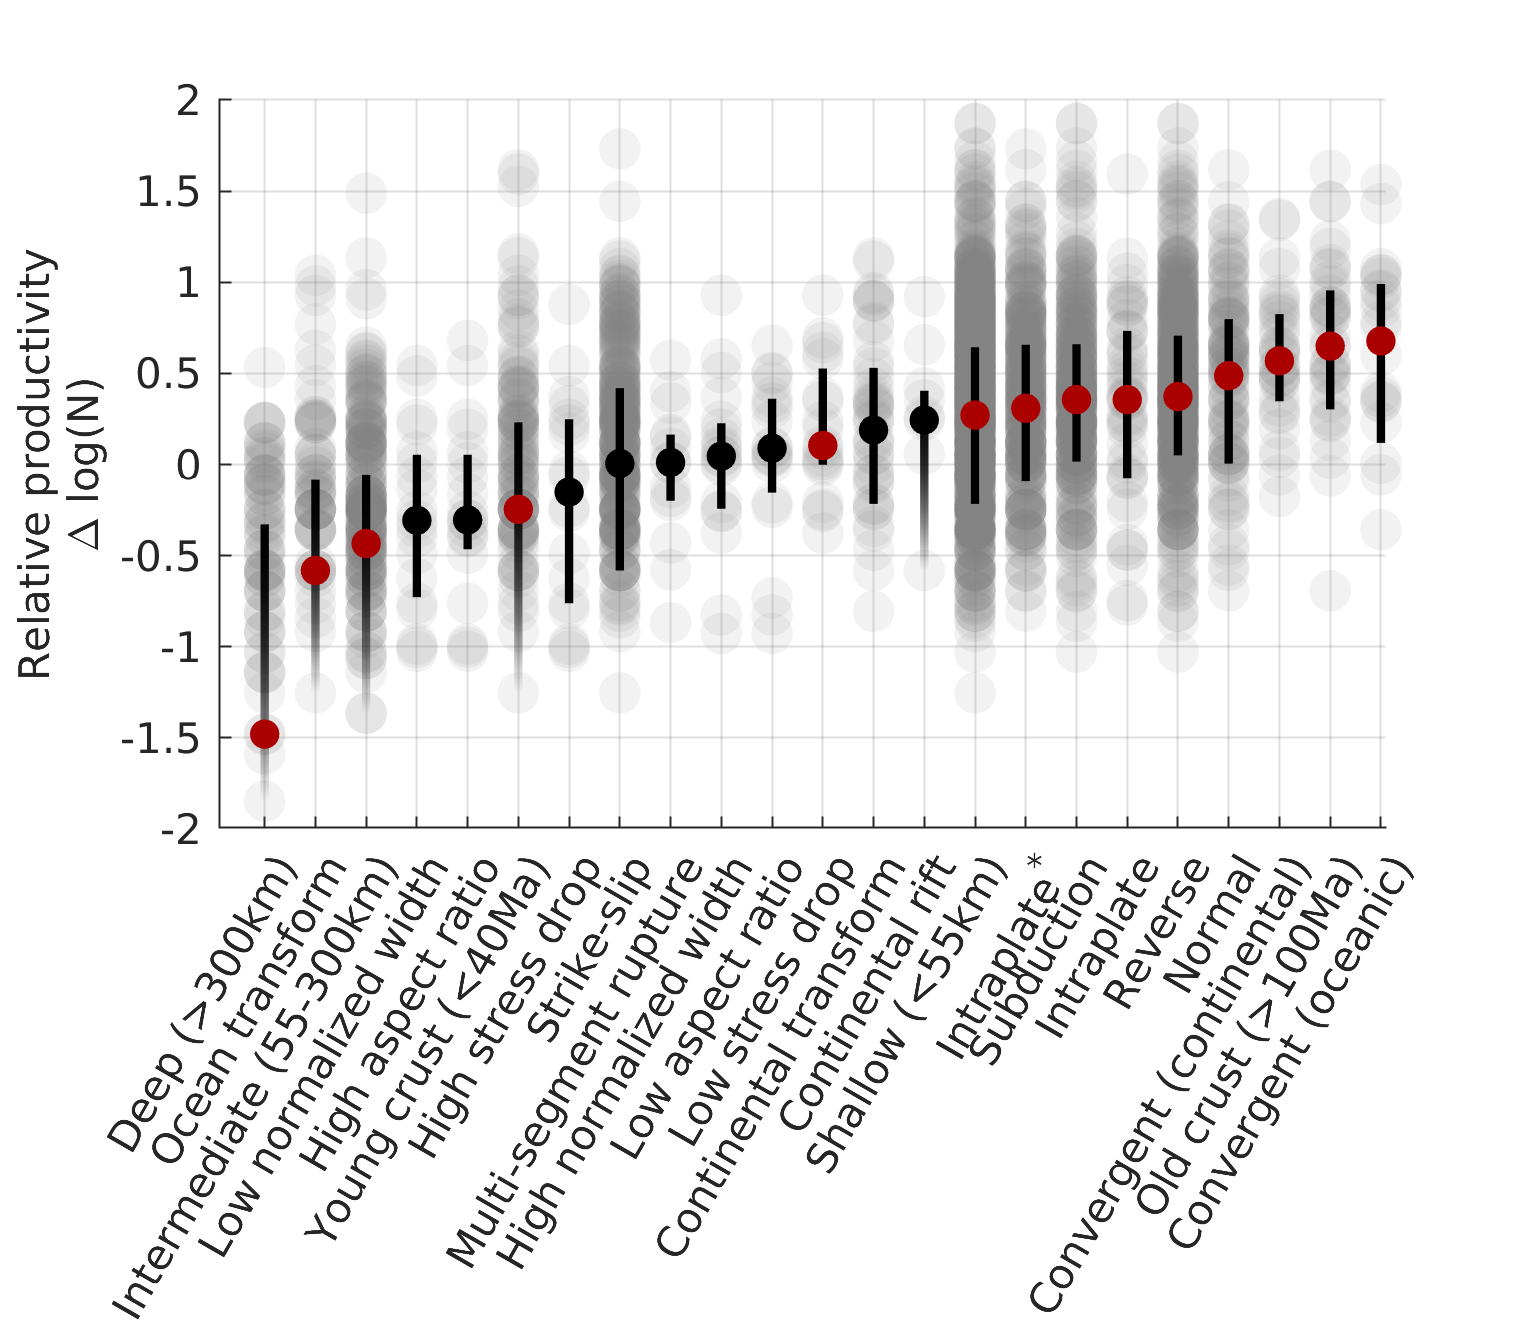
\includegraphics{cal_tech.png}
        \caption{Synthesis of relative productivity according to catalog subsets. The group considered here are the short list which best distinguished relative productivity based on our different lines of investigation (Sections \ref{sec:glob}-\ref{sec:source_parameters}). `High' and `low' subsets respectively refer to $>80$th and $<20$th percentile ranges of the data. Grey circles are individual mainshocks. Opaque points and error bars respectively indicate the median and interaquartile range of the subset. Fading error bars imply that mainshock sequences with no aftershocks are within the interquartile range of the data. \add{Attributes with red markers are consistent with the hypothesis that they are sample from a different continuous distribution than the overall population of earthquakes using a 2-sample Kolmogorov-Smirnov test at a 5\% significance threshold.}}
        \label{fig:caltech}
    \end{figure}

 \begin{figure}
    \centering
    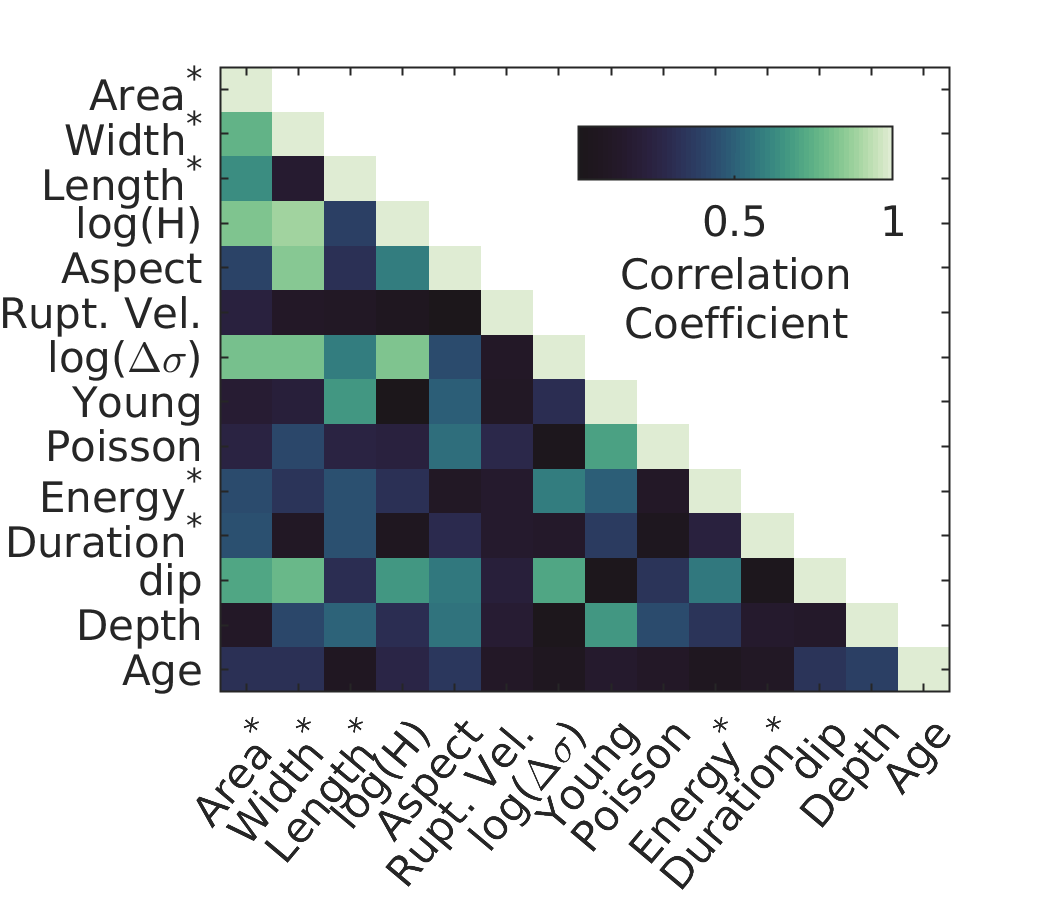
\includegraphics{covariance_plot.png}
    \caption{\add{Pearson Correlation Coefficient matrix for quantitative predictors of relative earthquake productivity. Correlation coefficients comprise earthquake shallower than 55~km for which all source attributes were calculated. Brighter colors indicate higher absolute values in correlation. Note that examining the correlation coefficient does not fully capture more non-linear interactions.}}
    \label{fig:covariance}
\end{figure}

\subsection{Importance of Fault Availability}

The dependence on crustal age, lithosphere type, depth, aspect ratio, stress drop, and the underlying magnitude scaling are all congruent with a primary physical control: \remove{the influence on aftershock productivity is the available volume of rock susceptible to brittle failure}\add{the volume of nearby rock susceptible to brittle failure influences aftershock productivity}. \remove{This consistency is perhaps the most significant result of this study.}

\remove{The increase in earthquake productivity with plate age is to the best of our knowledge a new finding.} Figure \ref{fig:caltech} places \change{this effect}{plate age} as the most pronounced control on aftershock statistics following depth effects. With increasing age, oceanic lithosphere becomes colder, thicker, more brittle and less buoyant. Subduction zone earthquakes hosted along younger lithosphere tend to generate larger earthquakes (lower b-values), particularly so in the first $\sim70$ Ma. \citet{Nishikawa2014EarthquakeBuoyancy} attributed the trend to changes in buoyancy of the subducting slab. While variations in b-value statistics may covary with aftershock productivity, we find it difficult to reconcile their physical interpretation with the increasing aftershock productivity along transform faults that we observe.

Old oceanic lithosphere is also thicker. Increasing the thickness of the lithosphere increases the volume in the brittle failing regime. Increasing the susceptibility of the surrounding volume to earthquakes stressing is a natural alternative explanation for the increased rate of aftershocks with plate age. Though the effect was more subdued, a careful analysis of subduction zones also revealed the same pattern \citep[Appendix of][]{Wetzler2016}. Old ($>100Ma$) oceanic lithosphere hosts seismicity along Japan and in the western Mediterranean Sea, which are highly productive in aftershocks (see Figure \ref{fig:global_res} for reference). Generally, the contrasting aftershock productivity of the Eastern and Western Pacific can be related to lithospheric age.

We may cast continental earthquakes, which we observe to have elevated aftershock productivity, as a highly thickened (old) lithosphere end member. Equivalently, convergent boundaries which effectively double the thickness of the lithosphere are associated with high aftershock productivity. The deeper the zone of low temperature brittle material, the higher the aftershock production.

Intermediate- and deep-focus earthquakes are the opposite end-member, instead exhibiting very low aftershock productivity. Deep earthquakes within subducting oceanic lithosphere are confined above and below by viscous mantle. Moreover the the lithosphere is caused to thin by thermal conduction from the warmer mantle. Subducting lithosphere becomes rejuvenated and hence aftershock poor.

Long aspect ratio ruptures reflect the saturation of the brittle crust which is limited in this case by the surface of the Earth above and by the ductile zone below \citep{Scholz2019}. Spatial confines limit the volume that may host aftershocks. It is telling to observe that the down-dip width of the rupture correlates far better with aftershock productivity than its the length (Figure \ref{fig:r2_finite_fault}). In other words, vertical confines (the surface and the ductile base of the seismogenic zone) are better controls on the productivity of earthquakes than the lateral limits.

The final evidence for the significance of volume availability arises from the scaling of aftershocks productivity with mainshock size. The scaling captures the mainshocks ability to activate a larger volume with increasing earthquake size. Our results are a natural extension of this basic premise. Fluctuations to the magnitude scaling, i.e. relative productivity, result from fluctuations in mainshocks ability to brittlely deform its surrounding volume.

\add{Previous work has found that clustering statistics correlate well with heat flow with high heat flow reducing aftershock productivity, and interpret their findings in the context of a temperature dependent rheology} \citep{Ben-Zion2006AnalysisRheology, Zaliapin2016AClusters}.\add{ The observations are consistent with fault availability playing an important role. Regions with thin lithosphere have high heat flow and so are predicted to be aftershock poor in both frameworks. However, the correlation of focal mechanism} (Figure \ref{fig:coloc}a) \add{with aftershock productivity is more challenging to explain by rheological changes alone. The direct correlation between aftershock productivity and heat flow may be a special case of the influence of fault availability since high heat flow can reduce the number of available faults for aftershocks.} %, however, other factors such as fault geometry can influence the fault availability as well.

\subsection{Improving Aftershock Forecasts}

Short term hazard assessment following a large earthquake relies on regional catalogs to calibrate the statistical behavior of the local seismicity. Unfortunately, seismic records are temporally limited and generally do not span large-earthquake-cycle timescales, particularly for the determination of aftershock parameters such as aftershock productivity. \add{For large events where local data is limited,} expert judgement will often rely on past ruptures to serve as analogs for the upcoming hazard. We extend and formalize this approach with a statistical treatment using flexible prediction tools. Using local analogs to determine the aftershock hazard is often impossible. Our analysis raises an complimentary approach. We in fact show that contextual attributes are strongly indicative of upcoming aftershock productivity. Thus, teleseismic data and a coarse knowledge of the local tectonic context can significantly help constrain short-term hazard following large earthquakes in poorly instrumented or quiescent areas. In particular, Figure \ref{fig:response}b suggests an algorithm to use in future aftershock prediction, \add{indicating up to 10-fold improvements in the forecast of aftershock counts.}

\section{Conclusion}

We synthesize multiple possible relationships between aftershock productivity and setting/source effects for earthquakes from 1990 to 2019. Global patterns suggest that earthquake productivity is particularly low along oceanic transform faults and tracks lithosphere ages. The functional relationship suggests that productivity increases because of the cooling and thickening of oceanic lithosphere with time. The rupture's aspect ratio, the down-dip width and, to a lesser degree, stress drop, correlate with aftershock productivity; other parameters including rupture duration, and length, scaled radiated energy and material parameters did not. Just a few parameters (plate age, dip, and normalized rupture area) are promising predictors of short-term seismicity forecast. Predictions do not require knowledge of the regional seismicity and therefore lend themselves well to large remote earthquakes where teleseismic data is available, but long term monitoring is not. Source geometry and the availability of stressed faults are inferred to provide primary control on the number of aftershocks triggered.

\acknowledgments
We would like to thank the members of the UCSC seismology laboratory for providing thoughtful insight and lively debate on the topic. Earthquake locations and magnitudes along with estimates of radiated energy were obtained from the IRIS data management center. Gavin Hayes provided all finite fault inversions. This work was fund by NSF-EAR Grant 1761987. To the best of our knowledge, no author has any conflict of interest publishing this research. \add{Finally, we thank the associate editor and the reviewers for their comments.}

\bibliography{references.bib}

\end{document}
